% !TEX root =  ../Dissertation.tex

\chapter{Results and Discussion}

In this section, it is presented a series of experiments done in different RL environments. Particularly, a 31-state simple GridWorld was used as proof of concept to analyze the efficient of our method by evaluating three keys problems in non-uniform sampling methods, such as task-agnostic sampling, outdated priorities, and state space coverage. After exploring these main issues, a general evaluation on slightly more complex was done to measure the performance of our algorithm in the RL scenario.

\section{Grid World - Episode Reward}

Episode Reward and Cumulative Reward were initially chosen to indicate the performance during training of different DQN extensions. The full priority weighting (weight: 1.0) version was used for BPERcn and BPERaa alternatives, such that it only prioritizes with bisimulation distances and not td-error. The algorithm was executed for 5 independent executions and the mean, min and max values (bottom and upper margin of shaded regions) per time steps are show in Figure \ref{fig:episode_cumulative_reward}. The methods DQN and DQN + MICO work as baseline to compare all other methods. 


Figure \ref{fig:episode_reward_grid_world} illustrates the episode reward per time steps during training, calculated in a 100 steps average window. While all methods show an improvement over time, converging after 100k steps, both BPERcn and BPERaa show promising improvements early in the training process, obtaining better performance than baselines and PER extension. However, over time, BPERaa keeps more consistent and stable improvements, indicating a better manage of priorities in the experience replay, while BPERcn shows a decrease of performance after the time step 30k. This results suggest that the smoother relative strategy 2, BPERaa, could in fact be beneficial in practice. Additionally, even though the GridWorld is a simple environment, the PER alternative under performs against all the other methods over time, showing the effectiveness of prioritizing behavioral dissimilar states.

The cumulative reward in Figure \ref{fig:cumulative_reward} helps us to check the overall time collected reward, a higher value will indicate a better ability to follow actions that leads to positive rewards. This complementary information indicates us that BPERaa in fact produces a policy that collect higher rewards, increasing the performance over the direct baseline DQN + MICO, which effectively show us that BPERaa is in fact making a positive effect in improving DQN + MICO. Alternatively, the other strategy, BPERcn, shows improvements in the earlier stages of learning, but eventually start decreasing the performance (around the 50k step) making the DQN + MICO reward acquisition worse, but keeping a similar performance that the baseline DQN. Overall, the PER alternative is the worse having difficulties to collect the rewards and in fact hindering the learning of the baseline DQN. 

\begin{figure}[h]
    \centering
    \begin{subfigure}{0.45\textwidth}
    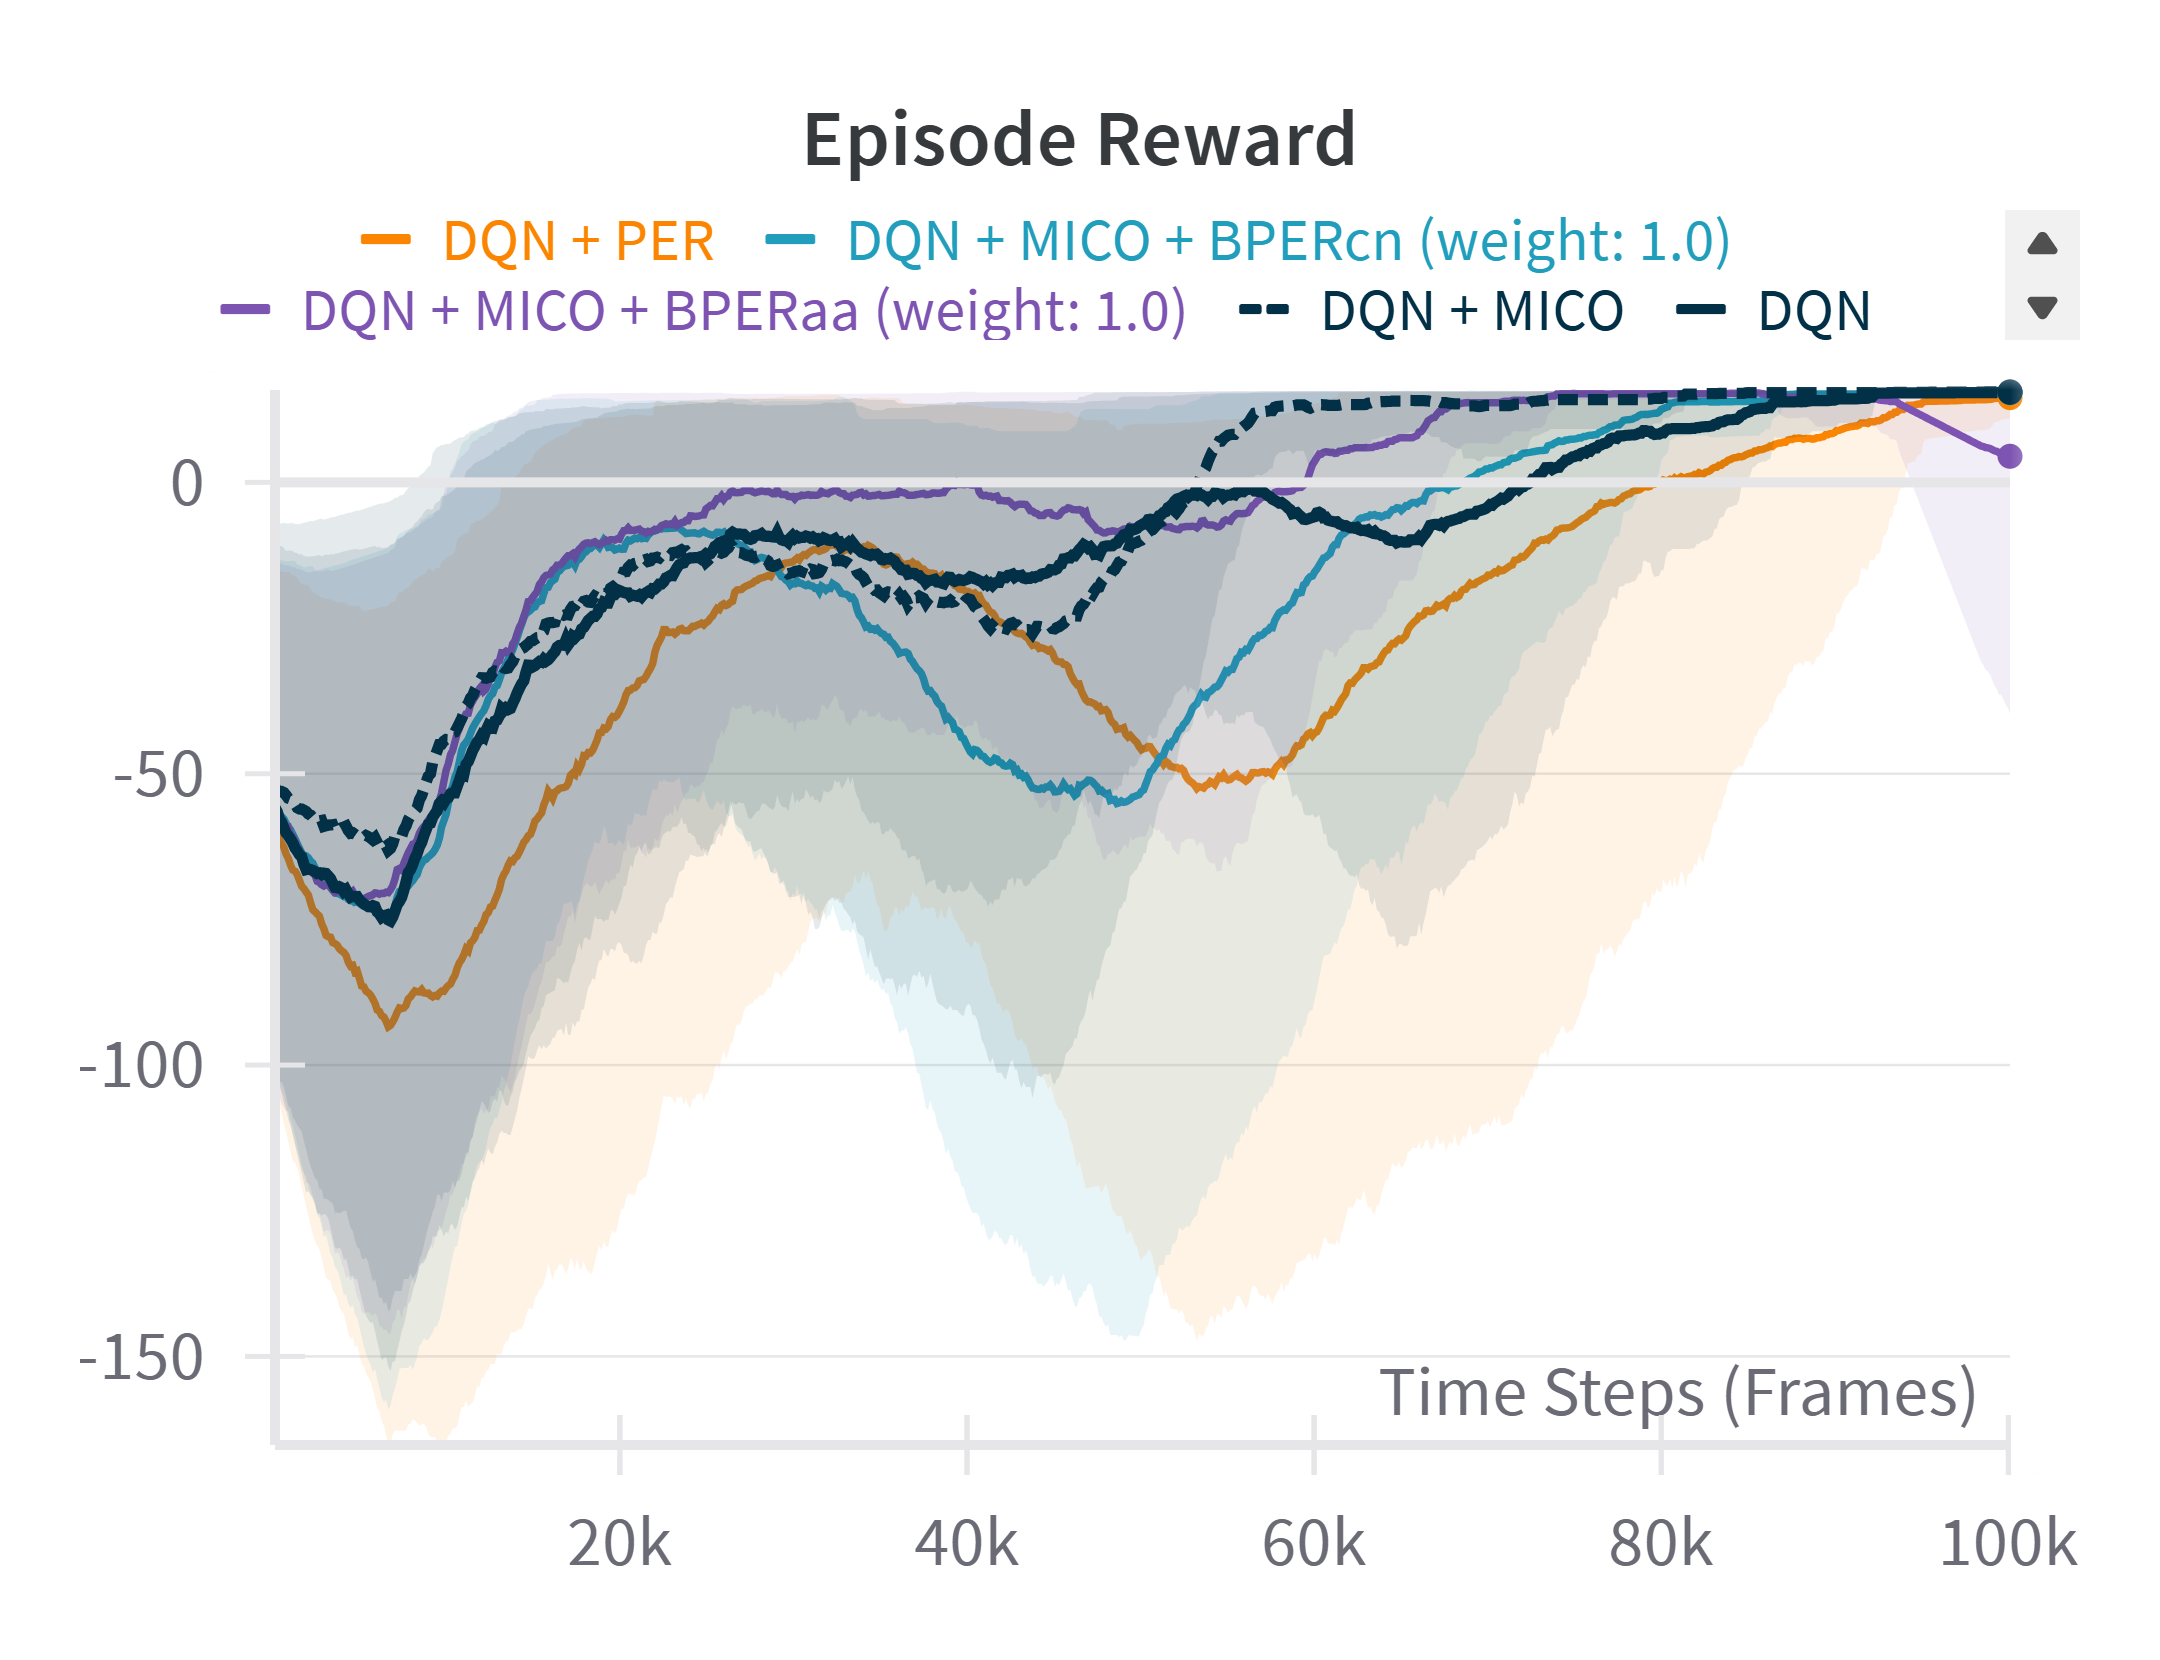
\includegraphics[width=\linewidth]{Results/grid_world/episode_reward_grid_world_window_100.png}
        \caption{Episode Reward}
        \label{fig:episode_reward_grid_world}
    \end{subfigure}
    \hfill
    \begin{subfigure}{0.45\textwidth}
        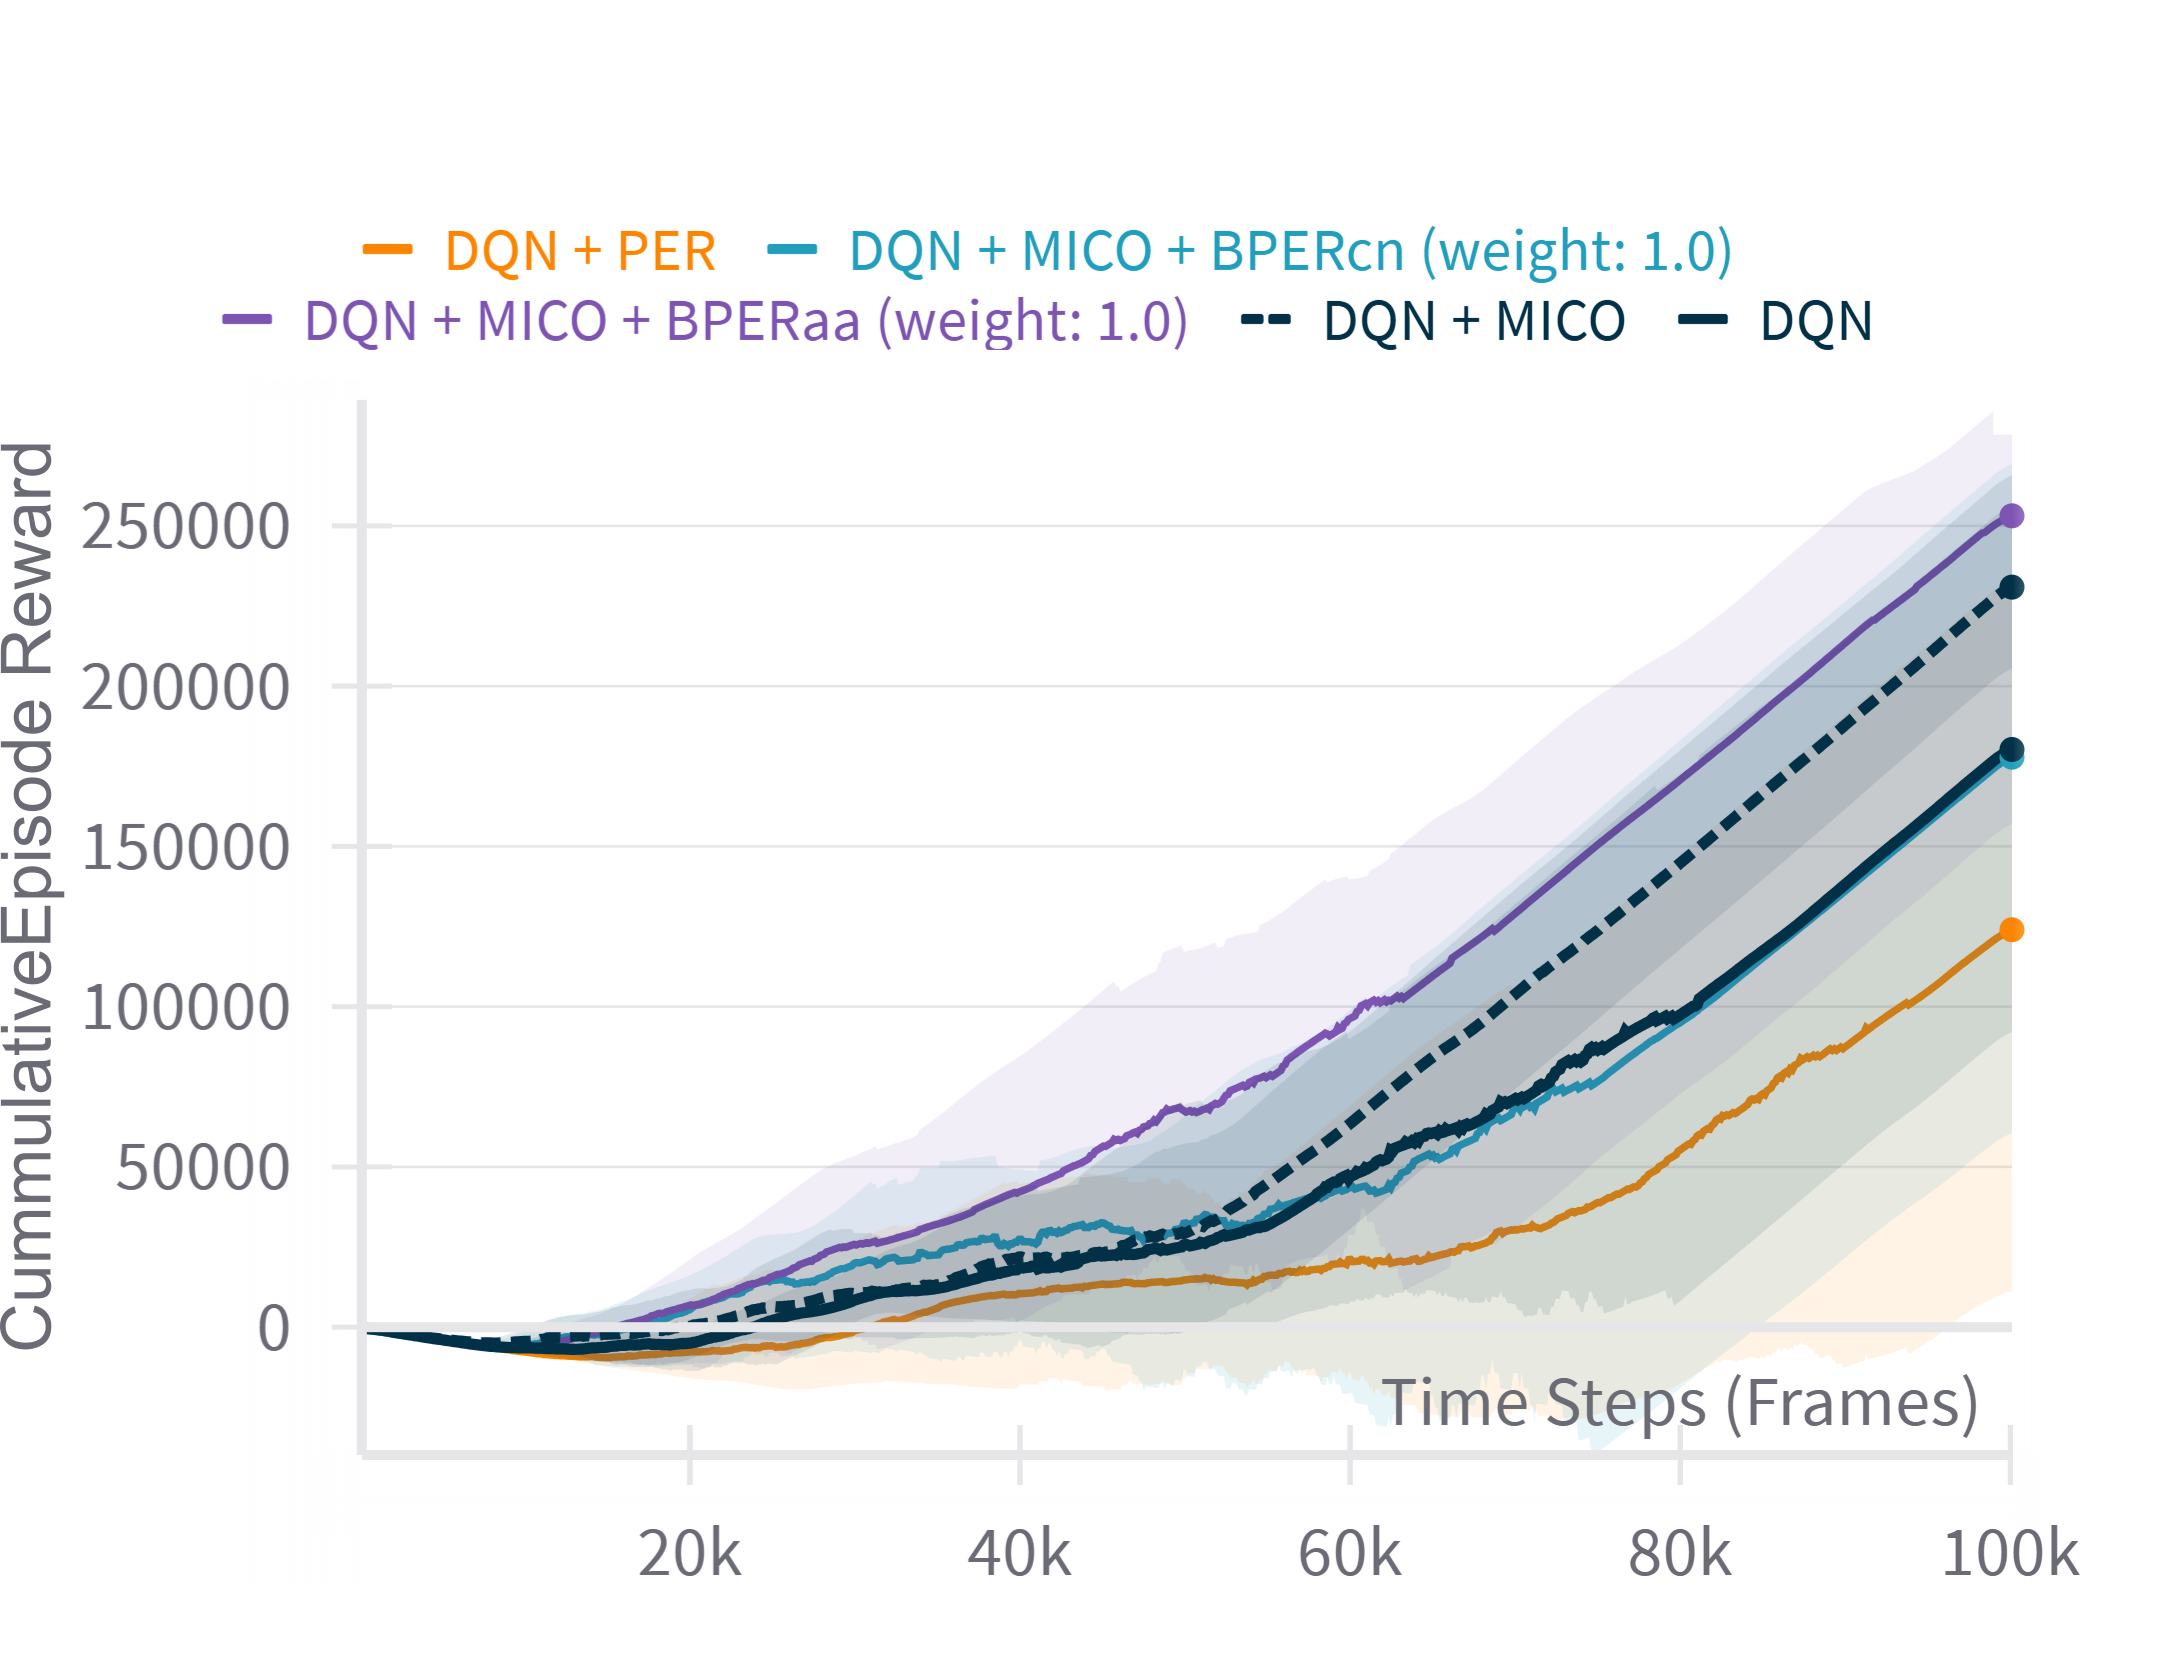
\includegraphics[width=\linewidth]{Results/grid_world/cumulative_episode_return.png}
        \caption{Cumulative Reward}
        \label{fig:cumulative_reward}
    \end{subfigure}
    \caption[Episode and Cumulative Reward]{\textbf{Episode and Cumulative Reward.} Reward performance comparison for different methods over time. The results represent the average from 5 independent executions, with shaded regions indicating the variability for each method.}
    \label{fig:cumulative_episode_reward}

\end{figure}


Exploring other perspective of the previous results, we proposed the episode reward gain to analyze more in detail the level of improvement of the proposed methods against our baselines (DQN and DQN + MICO). Figure \ref{fig:episode_reward_gain_dqn_and_mico} illustrates the Episode Reward gain on two different baselines, calculated on a window of 100 steps, and average over 5 independent executions. It is important to notice that only the mean values were used for the calculations. The results ratifies the excel improvements of BPERaa strategy over the other methods: BPERcn and PER againts both baselines, and showcases similar improvements of both bisimulation strategies in the earlier stages of the training. However, as mentioned before, this performance decreases in BPERcn around the step 30k. Under both baselines, the PER method underperform enormously by hinder the proper learning of the policy.

\begin{figure}[h]
    \centering
    \begin{subfigure}{0.45\textwidth}
    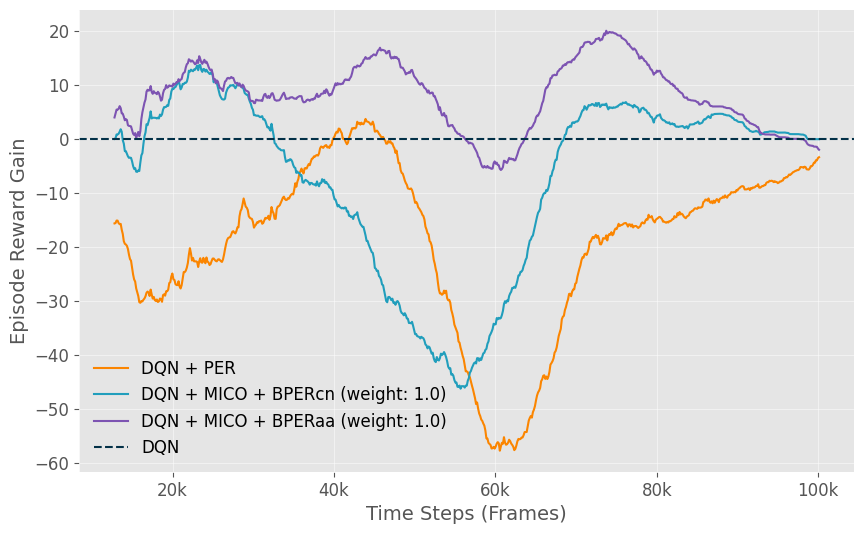
\includegraphics[width=\linewidth]{Results/grid_world/episode_reward_gain_baseline_dqn.png}
        \caption{Baseline DQN}
        \label{fig:episode_reward_gain_dqn}
    \end{subfigure}
    \hfill
    \begin{subfigure}{0.45\textwidth}
        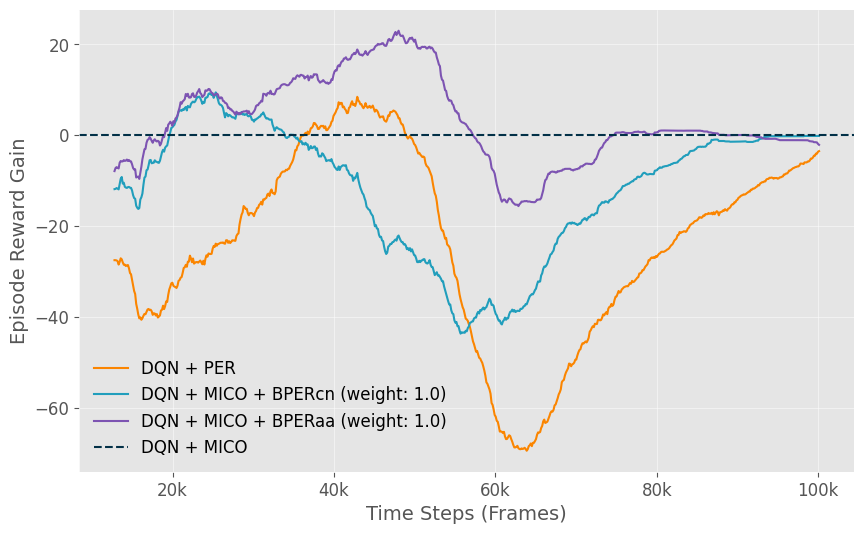
\includegraphics[width=\linewidth]{Results/grid_world/episode_reward_gain_baseline_dqn_mico.png}
        \caption{Baseline DQN + MICO}
        \label{fig:episode_reward_gain_dqn_mico}
    \end{subfigure}
    \caption{Episode Reward Gain }
    \label{fig:episode_reward_gain_dqn_and_mico}
\end{figure}

\section{Task-agnostic Sampling}

In this section, the intention is empirically demonstrate that the proposed method takes into account the behavior for prioritized samples efficiently. To do that, we require a way to quantitatively evaluated how many behavioral dissimilar transitions there are in the current experience replay. Specifically, the on-policy bisimulation recurrent operator $T_K^\pi$ for deterministic environments (see Equation \ref{eq:deterministic_on_policy_bisimulation_metric}) allow us to calculate exact on-policy bisimulation distances. Then, each transition in the experience replay can be associated with a exact bisimulation distance between the current and next state, effectively providing a behavioral value per transition, and allowing us to evaluate the level of behavioral similar or dissimilar transitions in an experience replay. 

Figure \ref{fig:exact_bisimulation_distributions} illustrates the distribution over the exact current-next on-policy bisimulation distances in the experience replay over time. In the strategies BPERcn and BPERaa, the behavioral dissimilar transitions evolve to larger values than PER over time, clearly demonstrating how our method will prioritized more frequently those larger behavioral dissimilar transitions. As the BPERcn encourages highly dissimilar transition between the current and next states approximated in the loop, the results from Figure \ref{fig:exact_bisim_bpercn} are expected. However, a more interesting result is that despite of BPERaa prioritized the transition based on a relative priority to the current mini-batch, this second strategy is still able to prioritize dissimilar experience as efficiently as the strategy BPERcn (see Figure \ref{fig:exact_bisim_bperaa}).

Another interesting result is that even though the method aims to prioritized highlight dissimilar transitions, Figures \ref{fig:exact_bisimulation_distributions} still show a lot of transitions with exact bisimilar distance close to zero, possible coming from the nature of the environment that contains highly similar states.

This result suggest that despite of the td-error is an indicator of possible improvement over the q-values, this is not enough to define a the expected learning improving and in this scenario a notion of behavioral similarity works better as an indicator of expected learning improving.


\begin{figure}[h]
    \centering
    \begin{subfigure}{0.32\textwidth}
    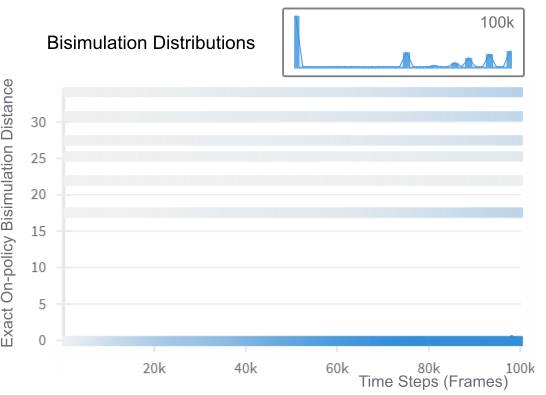
\includegraphics[width=\linewidth]{Results/grid_world/exact_bisimulation_dqn_per.png}
        \caption{DQN + PER}
        \label{fig:exact_bisim_per}
    \end{subfigure}
    \hfill
    \begin{subfigure}{0.32\textwidth}
        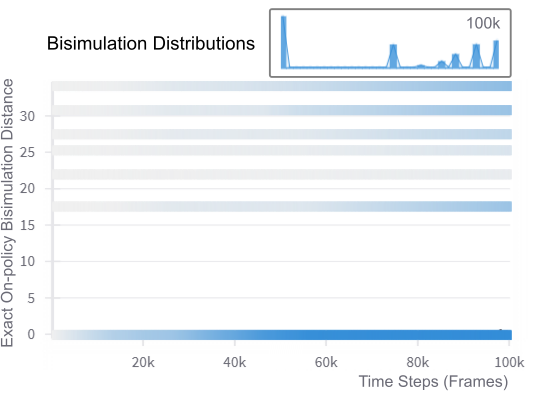
\includegraphics[width=\linewidth]{Results/grid_world/exact_bisimulation_dqn_mico_bpercn.png}
        \caption{DQN (MICO) + BPERcn}
        \label{fig:exact_bisim_bpercn}
    \end{subfigure}
    \hfill
    \begin{subfigure}{0.32\textwidth}
        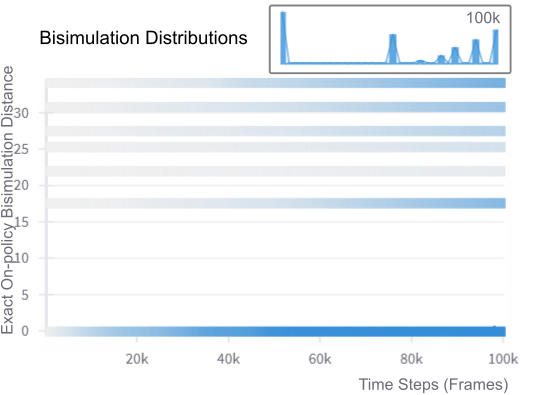
\includegraphics[width=\linewidth]{Results/grid_world/exact_bisimulation_dqn_mico_bperaa.png}
        \caption{DQN (MICO) + BPERaa}
        \label{fig:exact_bisim_bperaa}
    \end{subfigure}
    \caption{Two images side-by-side}
    \label{fig:exact_bisimulation_distributions}
\end{figure}

\begin{figure}[h]
    \centering
    \begin{subfigure}{0.32\textwidth}
    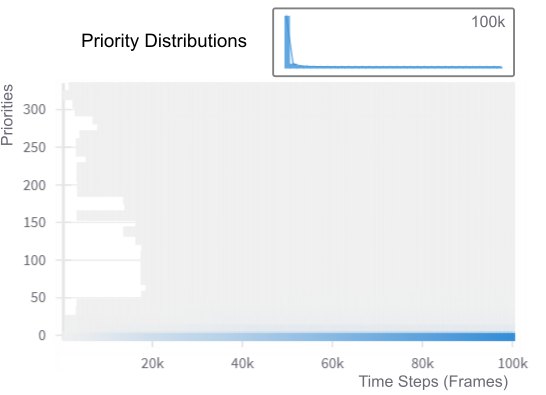
\includegraphics[width=\linewidth]{Results/grid_world/priority_distribution_dqn_per.png}
        \caption{DQN + PER}
        \label{fig:on_policy_weighting}
    \end{subfigure}
    \hfill
    \begin{subfigure}{0.32\textwidth}
        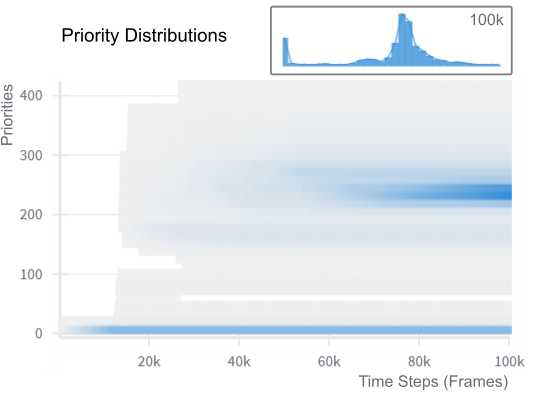
\includegraphics[width=\linewidth]{Results/grid_world/priority_distribution_dqn_mico_bpercn.png}
        \caption{DQN (MICO) + BPERcn}
        \label{fig:uniform_weighting}
    \end{subfigure}
    \hfill
    \begin{subfigure}{0.32\textwidth}
        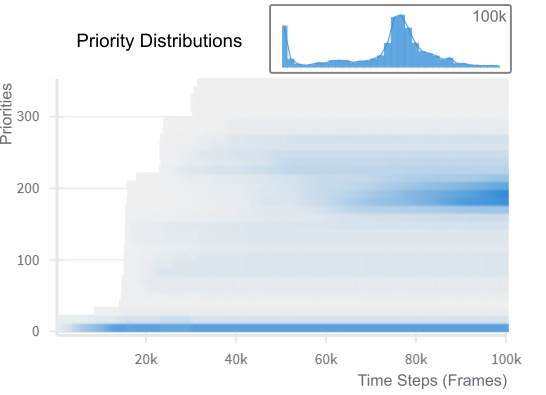
\includegraphics[width=\linewidth]{Results/grid_world/priority_distribution_dqn_mico_bperaa.png}
        \caption{DQN (MICO) + BPERaa}
        \label{fig:uniform_weighting}
    \end{subfigure}
    \caption{Two images side-by-side}
    \label{fig:outdated_priorities}
\end{figure}



\begin{figure}[h]
    \centering
    \begin{subfigure}{1.\textwidth}
    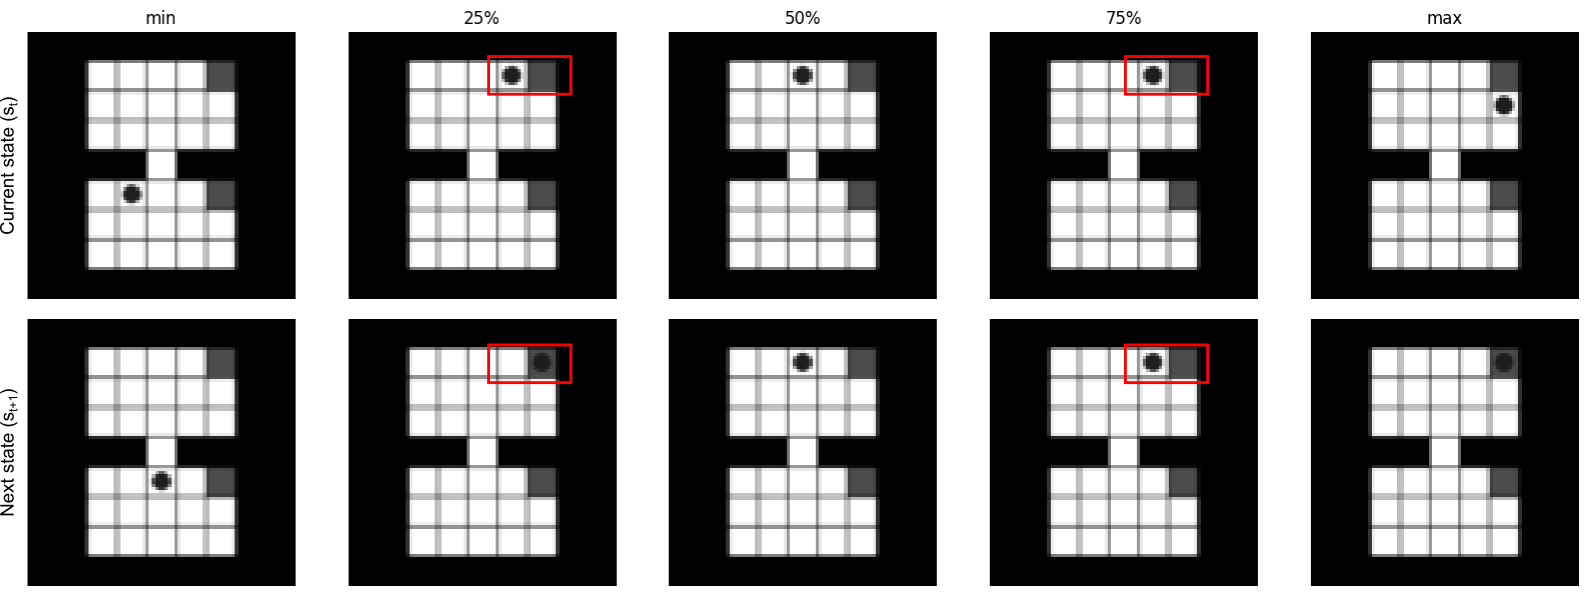
\includegraphics[width=\linewidth]{Results/grid_world/quartiles_images_per.png}
        \caption{DQN + PER}
        \label{fig:on_policy_weighting}
    \end{subfigure}
    \hfill
    \begin{subfigure}{1.\textwidth}
        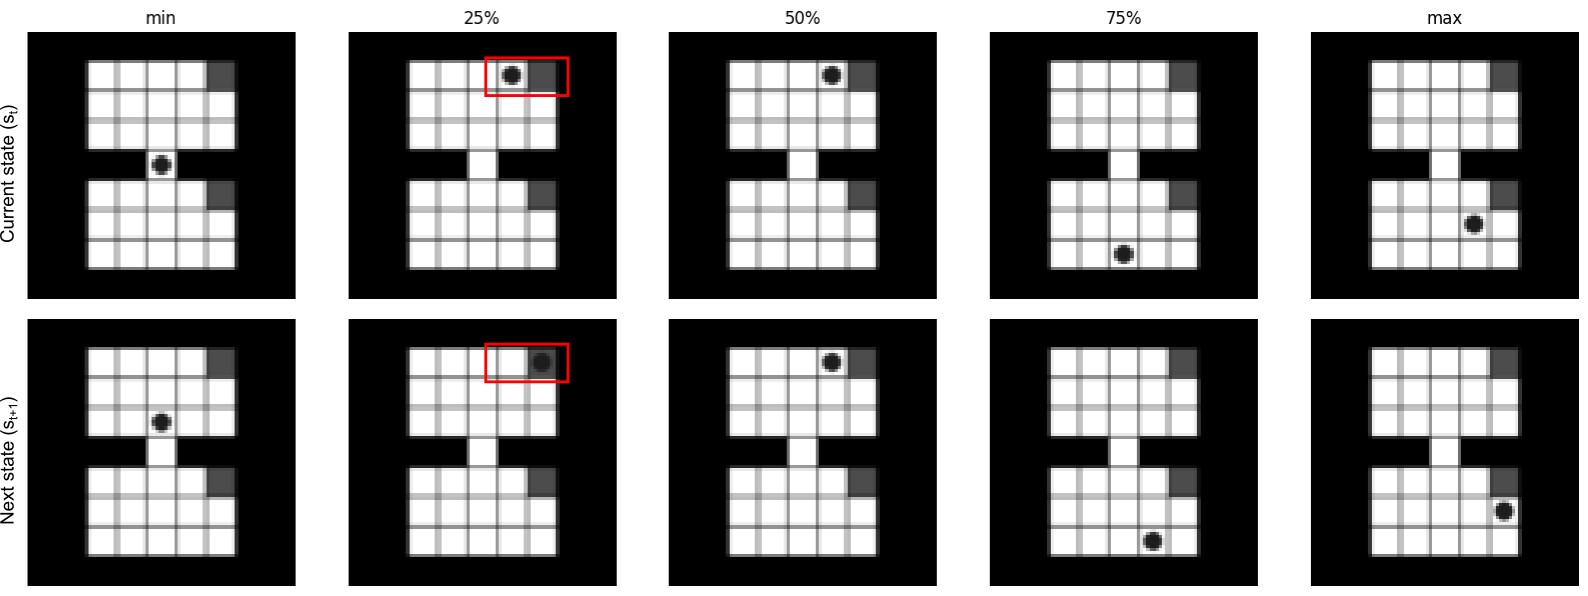
\includegraphics[width=\linewidth]{Results/grid_world/quartiles_images_dqn_mico_bpercn.png}
        \caption{DQN (MICO) + BPERcn}
        \label{fig:uniform_weighting}
    \end{subfigure}
    \hfill
    \begin{subfigure}{1.\textwidth}
        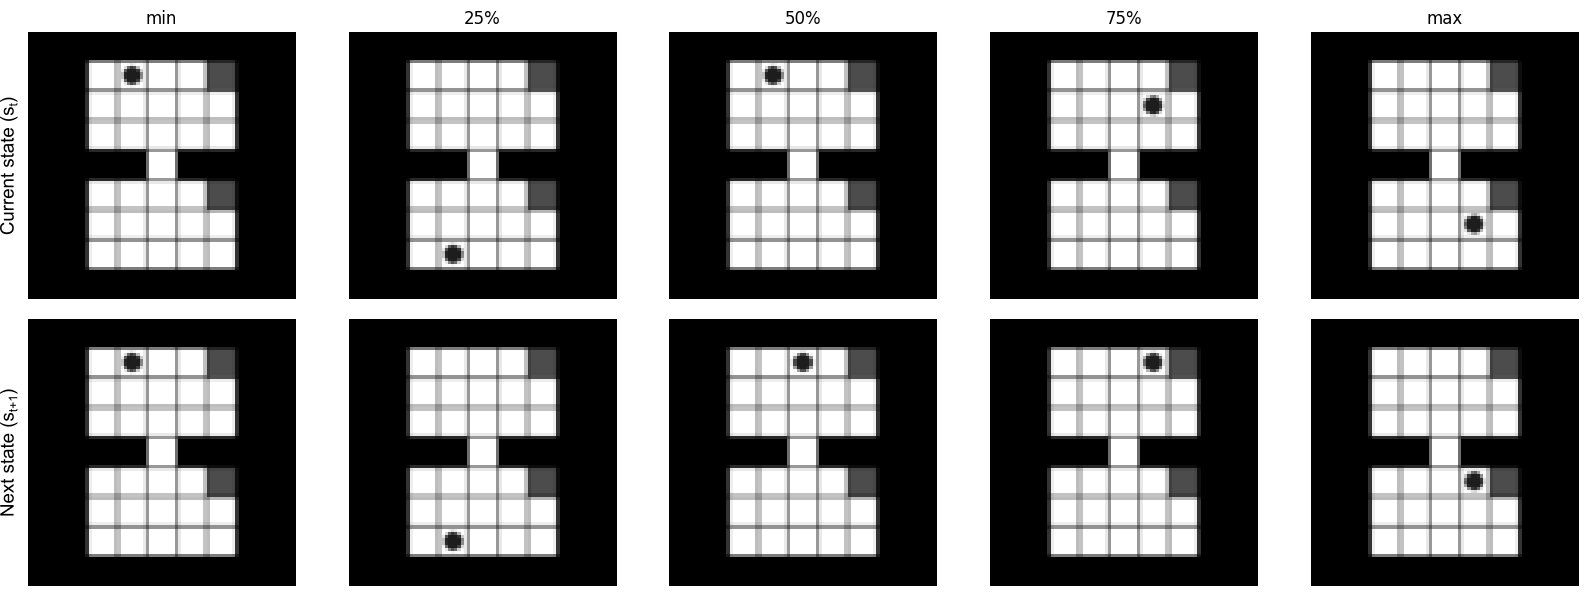
\includegraphics[width=\linewidth]{Results/grid_world/quartiles_images_dqn_mico_bperaa.png}
        \caption{DQN (MICO) + BPERaa}
        \label{fig:uniform_weighting}
    \end{subfigure}
    \caption{Two images side-by-side}
    \label{fig:outdated_priorities}
\end{figure}


\section{Outdated Priorities}

\begin{figure}[h]
    \centering
    \begin{subfigure}{0.45\textwidth}
    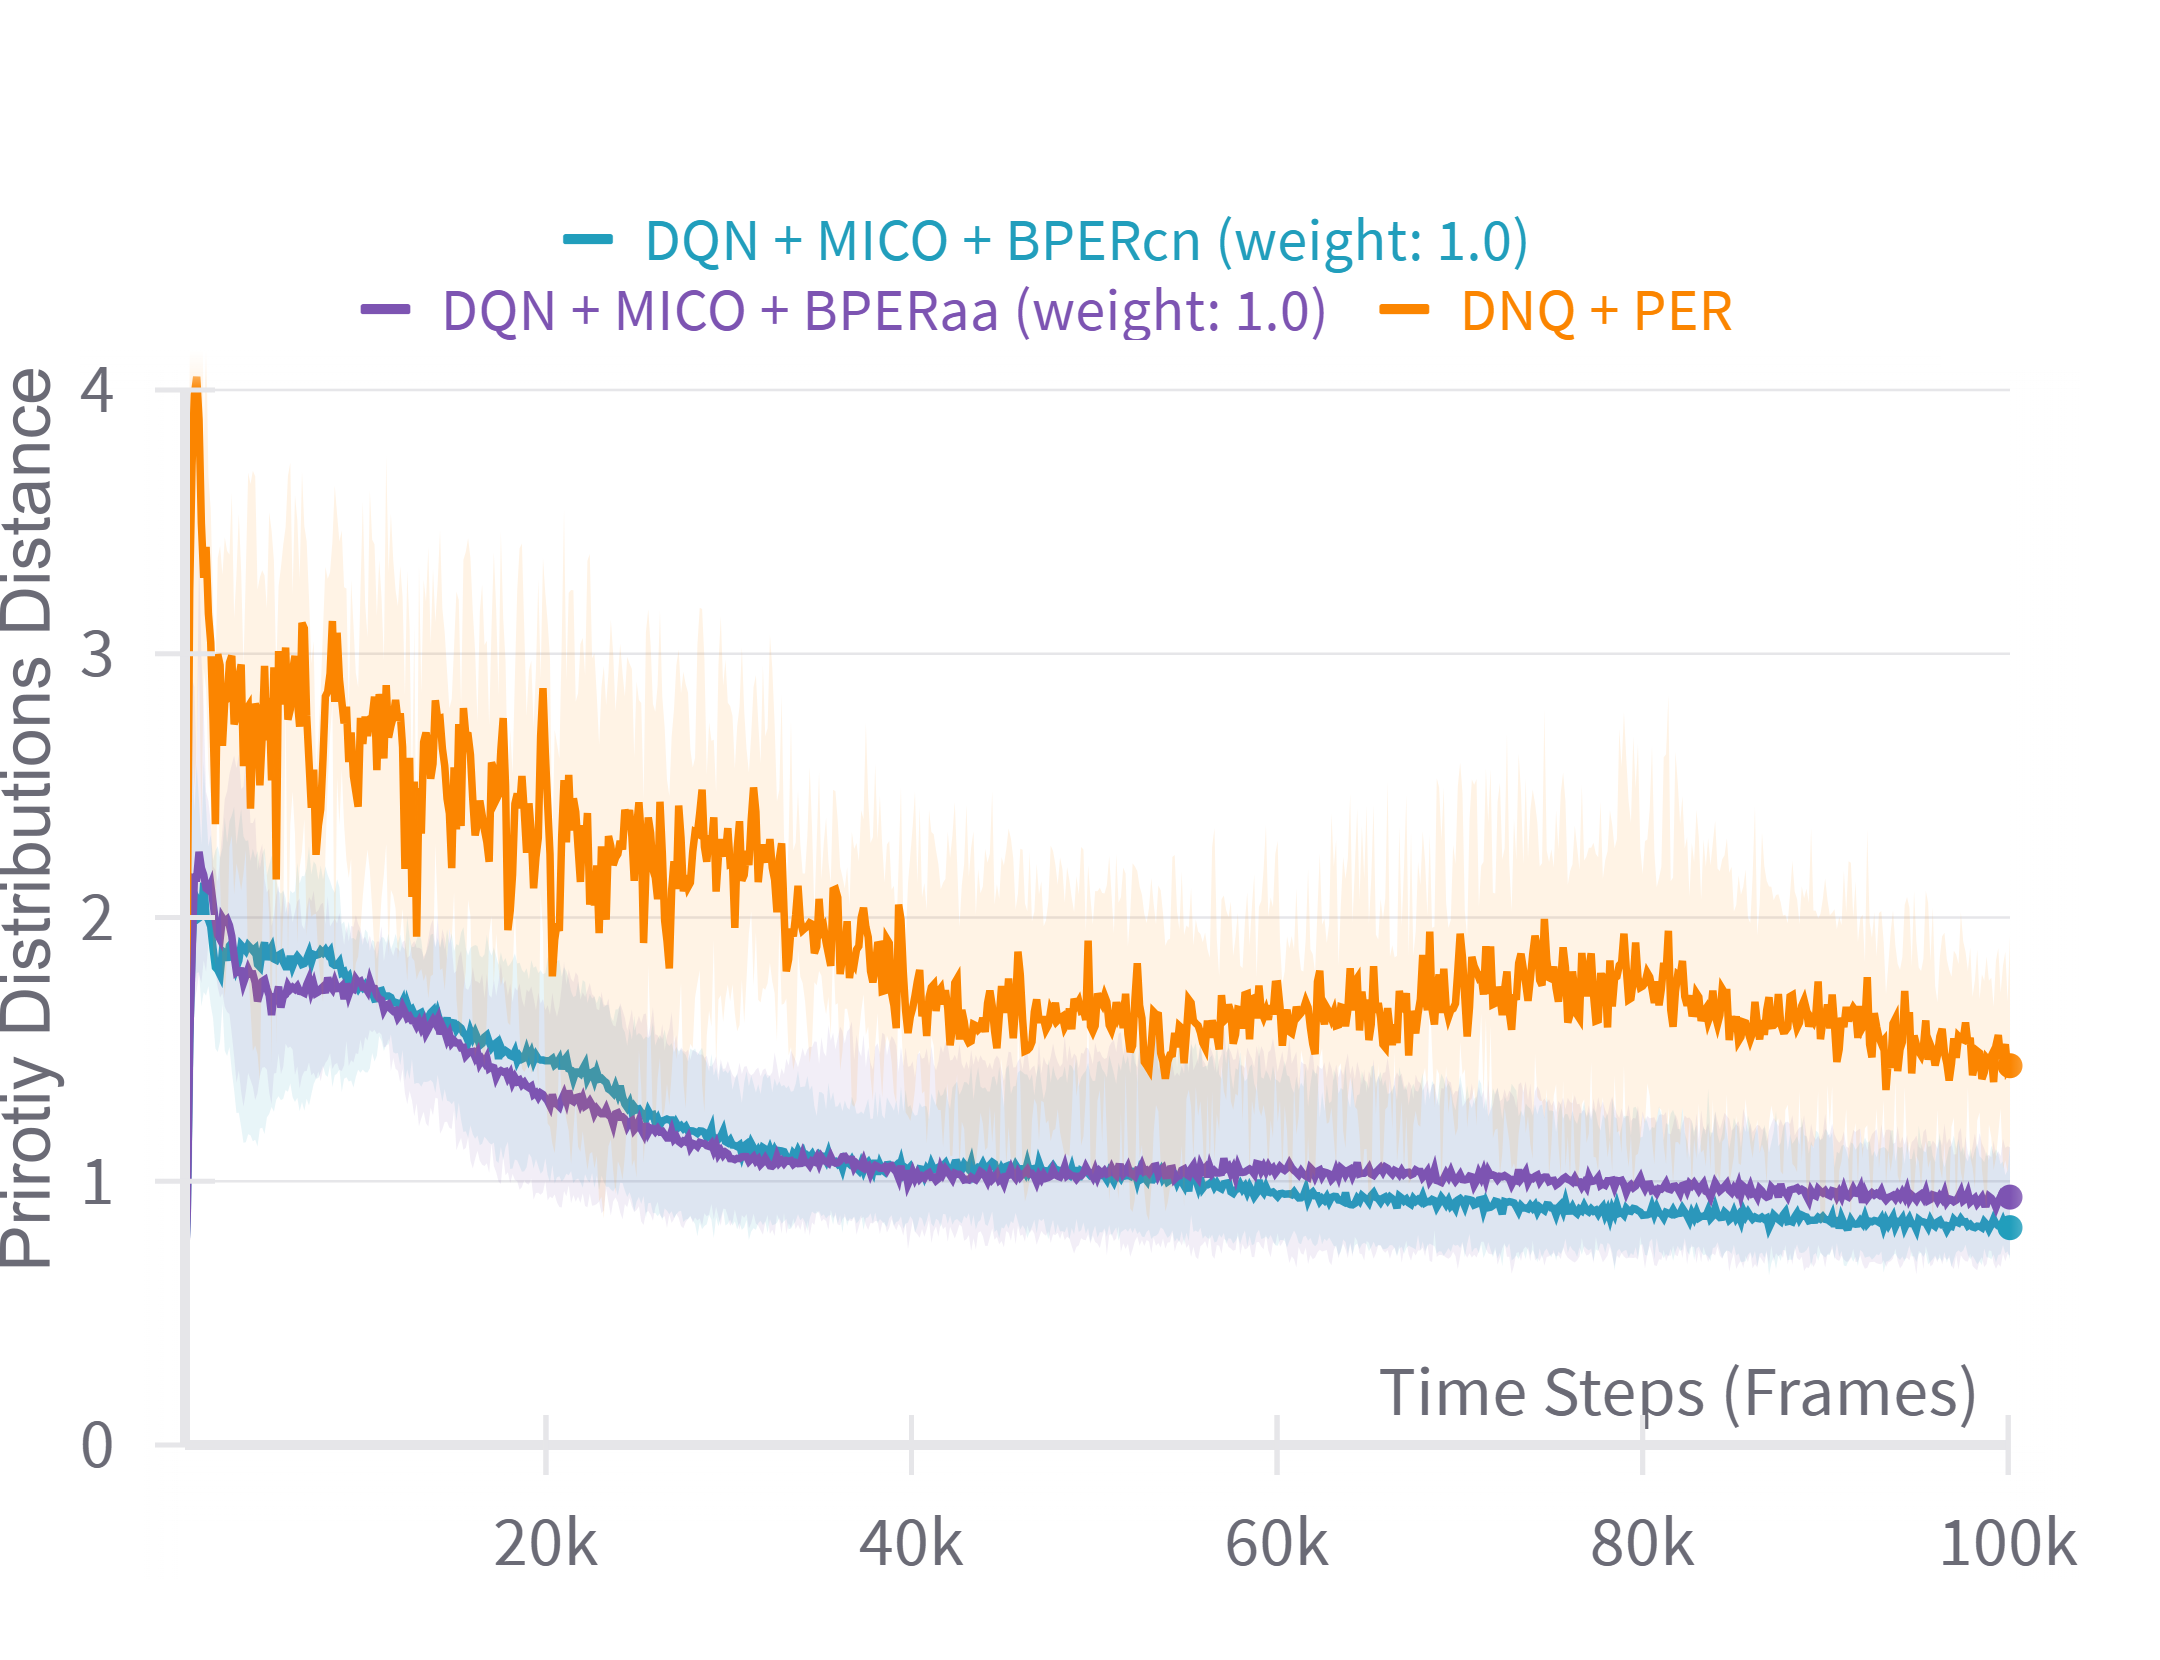
\includegraphics[width=\linewidth]{Results/grid_world/on_policy_weighting_outdated_priorities.png}
        \caption{On-policy Weighting}
        \label{fig:on_policy_weighting}
    \end{subfigure}
    \hfill
    \begin{subfigure}{0.45\textwidth}
        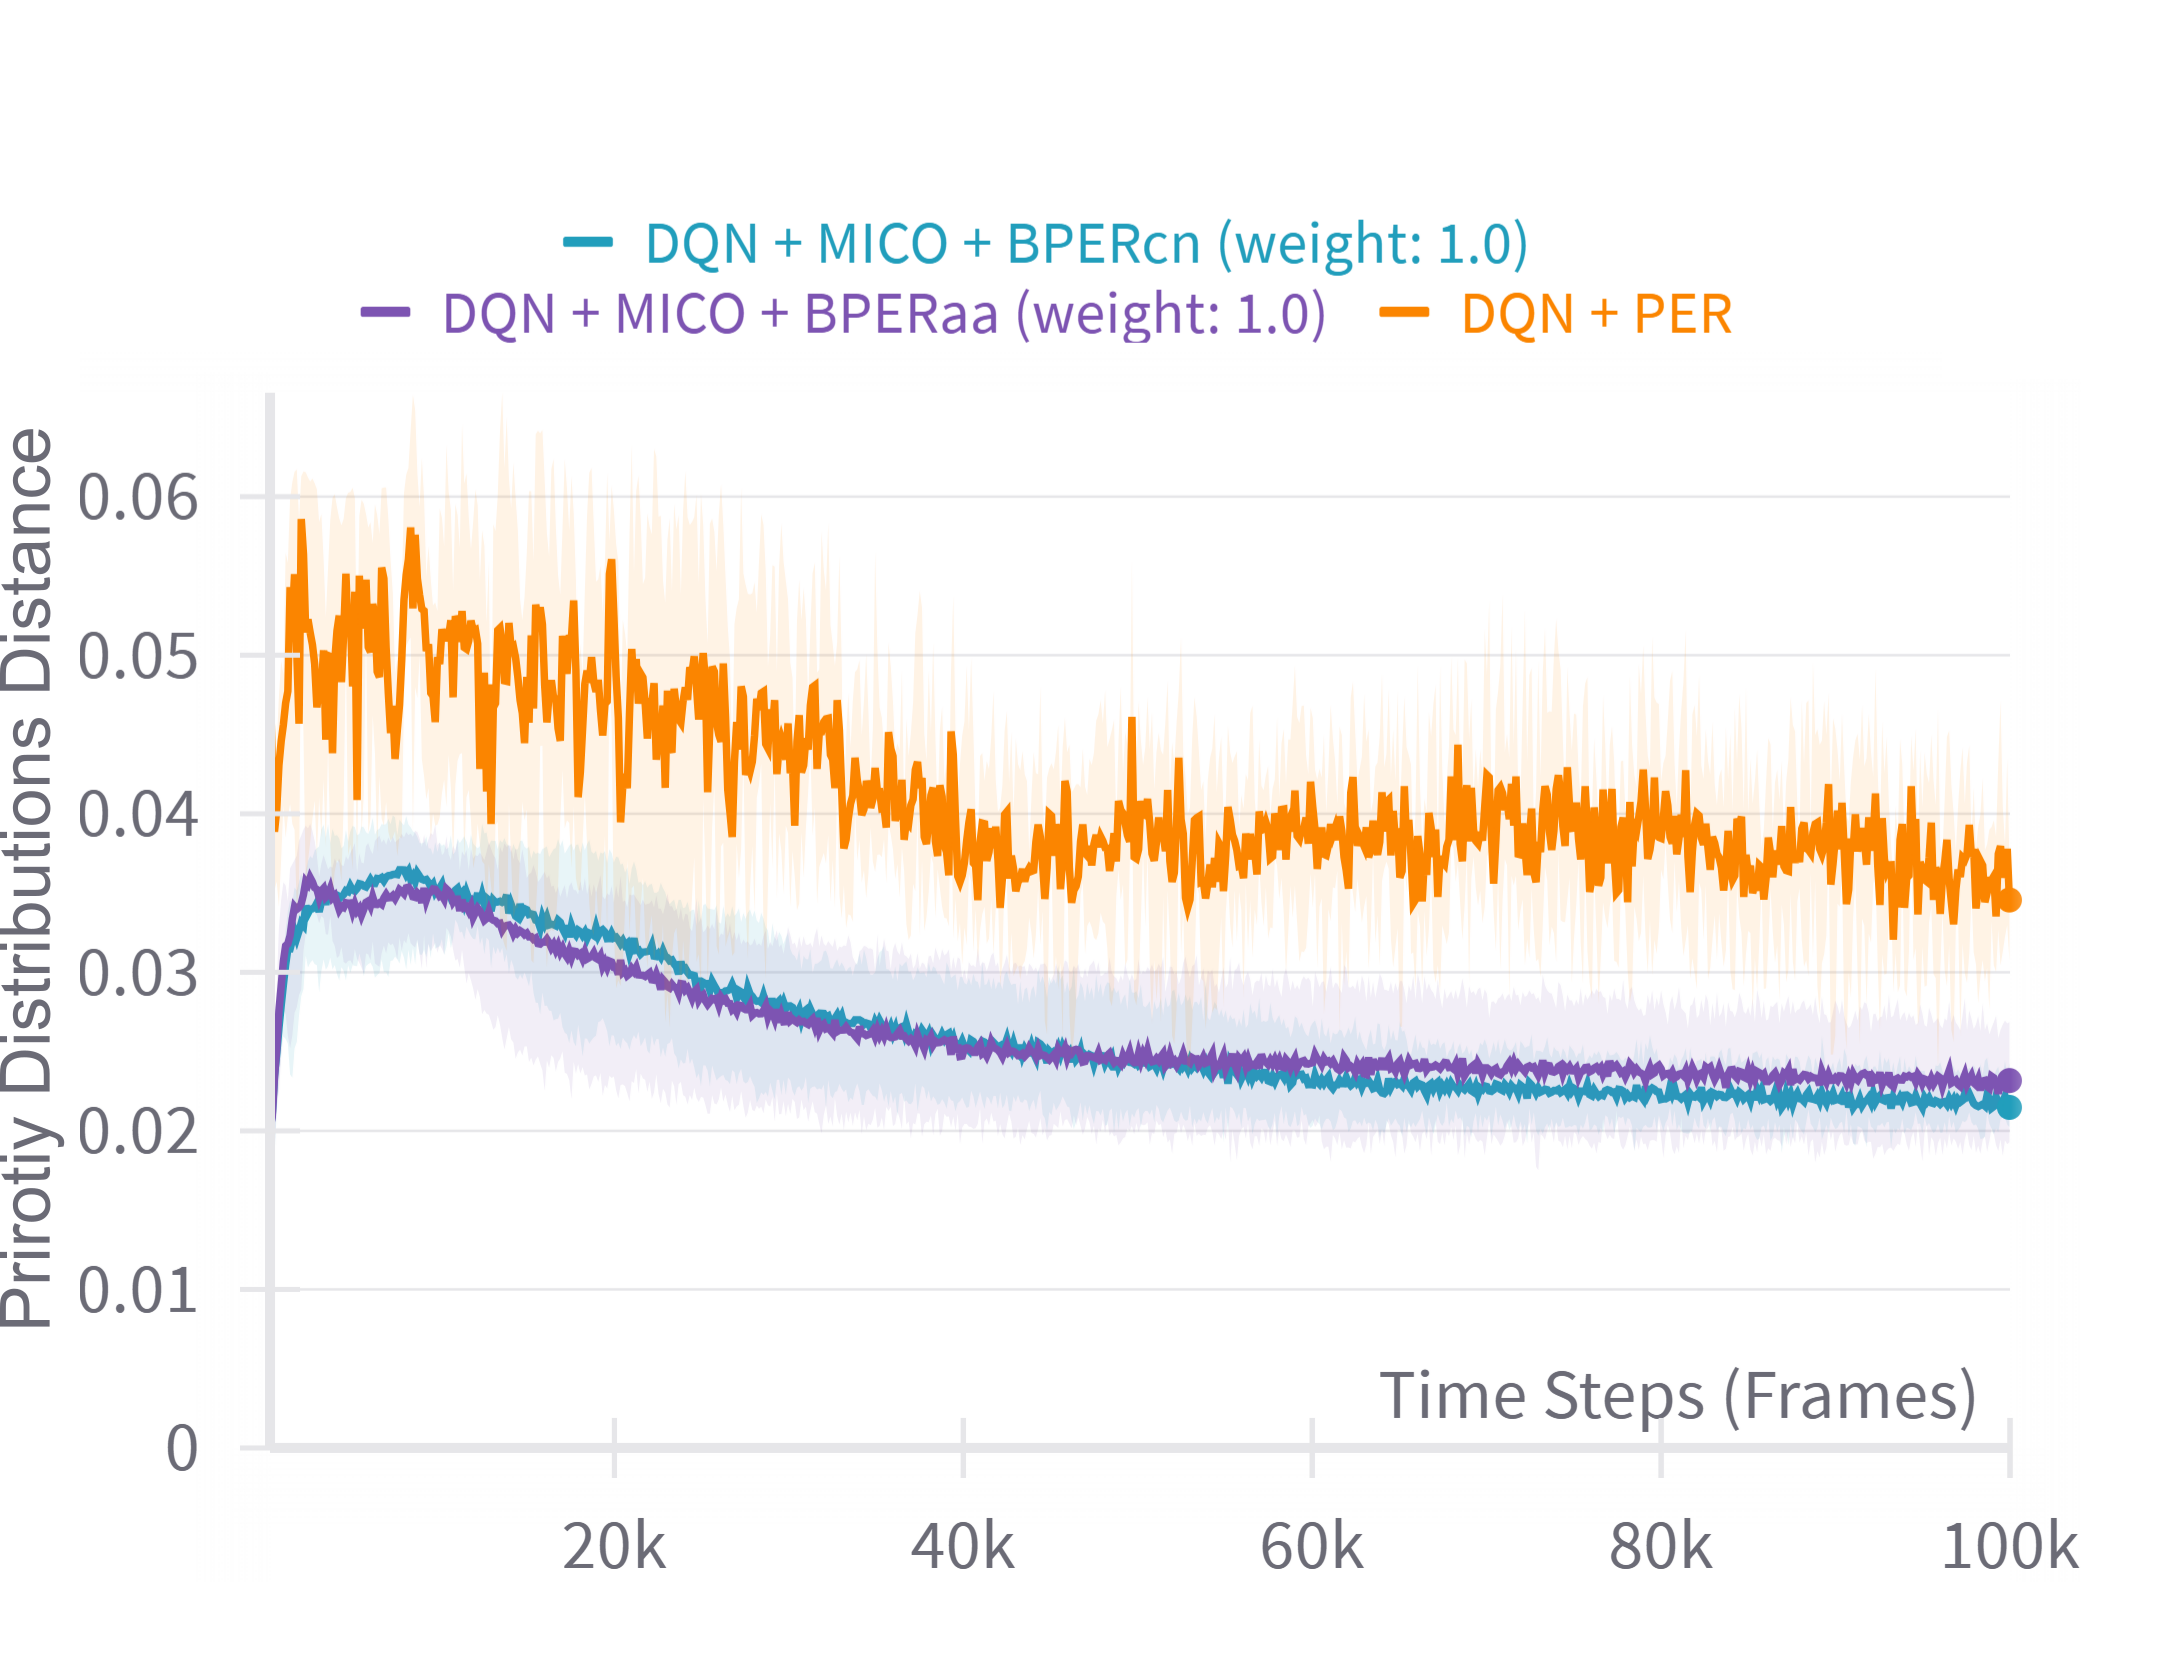
\includegraphics[width=\linewidth]{Results/grid_world/uniform_weighting_outdated_priorities.png}
        \caption{Uniform Weighting}
        \label{fig:uniform_weighting}
    \end{subfigure}
    \caption{Two images side-by-side}
    \label{fig:outdated_priorities}
\end{figure}



\section{State Space Coverage}

\begin{figure}[h]
    \centering
    % Add horizontal space to center the first two subfigures
    \hspace*{\fill}
    \begin{subfigure}{0.45\textwidth}
        \centering % Center the individual subfigure
        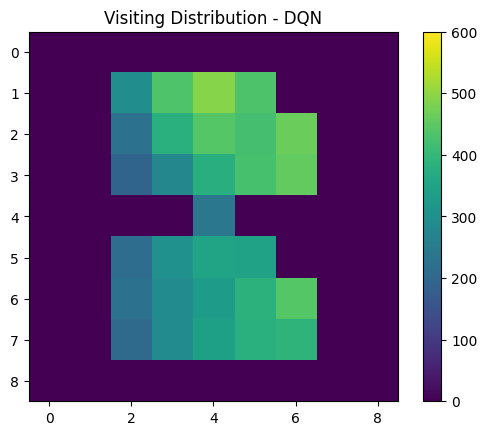
\includegraphics[width=0.70\linewidth]{Results/grid_world/visitation_distribution_dqn.png}
        \caption{DQN}
        \label{fig:on_policy_weighting}
    \end{subfigure}
    \hspace*{\fill} % Adjust space between subfigures
    \begin{subfigure}{0.45\textwidth}
        \centering % Center the individual subfigure
        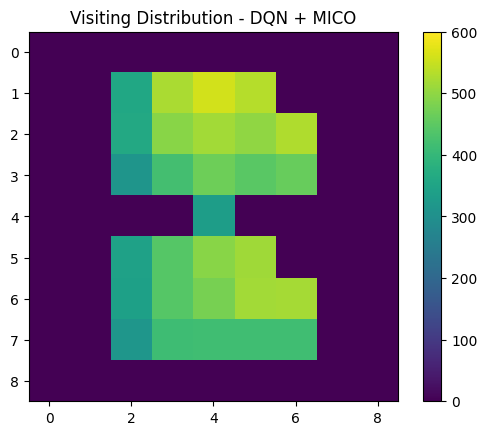
\includegraphics[width=0.70\linewidth]{Results/grid_world/visitation_distribution_dqn_mico.png}
        \caption{DQN + MICO}
        \label{fig:uniform_weighting}
    \end{subfigure}
    \hspace*{\fill} % Add horizontal space to center the first two subfigures
    \vfill
    \begin{subfigure}{0.32\textwidth}
        \centering
        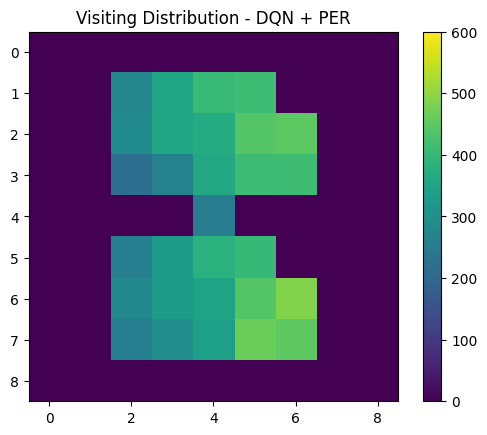
\includegraphics[width=\linewidth]{Results/grid_world/visitation_distribution_dqn_per.png}
        \caption{DQN + PER}
        \label{fig:uniform_weighting_2}
    \end{subfigure}
    \hfill
    \begin{subfigure}{0.32\textwidth}
        \centering
        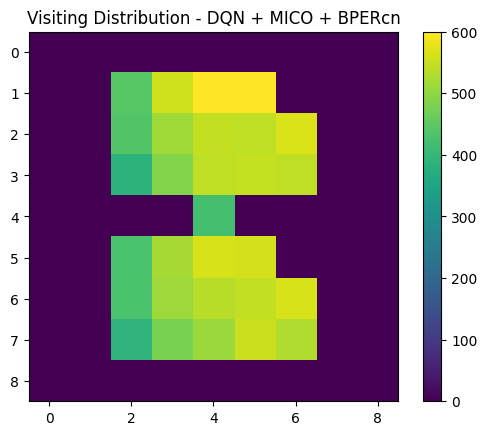
\includegraphics[width=\linewidth]{Results/grid_world/visitation_distribution_dqn_mico_bpercn.png}
        \caption{DQN + MICO + BPERcn}
        \label{fig:uniform_weighting_3}
    \end{subfigure}
    \hfill
    \begin{subfigure}{0.32\textwidth}
        \centering
        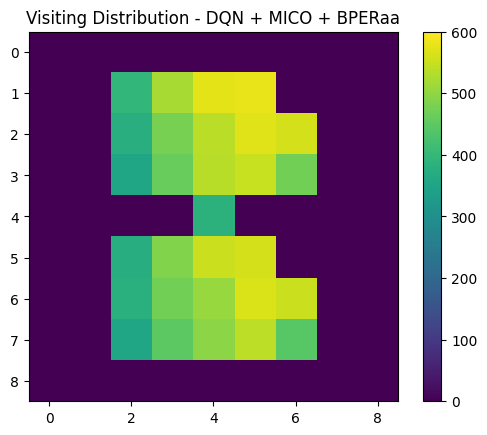
\includegraphics[width=\linewidth]{Results/grid_world/visitation_distribution_dqn_mico_bperaa.png}
        \caption{DQN + MICO + BPERaa}
        \label{fig:uniform_weighting_4}
    \end{subfigure}
    \caption{Two images side-by-side}
    \label{fig:outdated_priorities}
\end{figure}


\begin{figure}
    \centering
    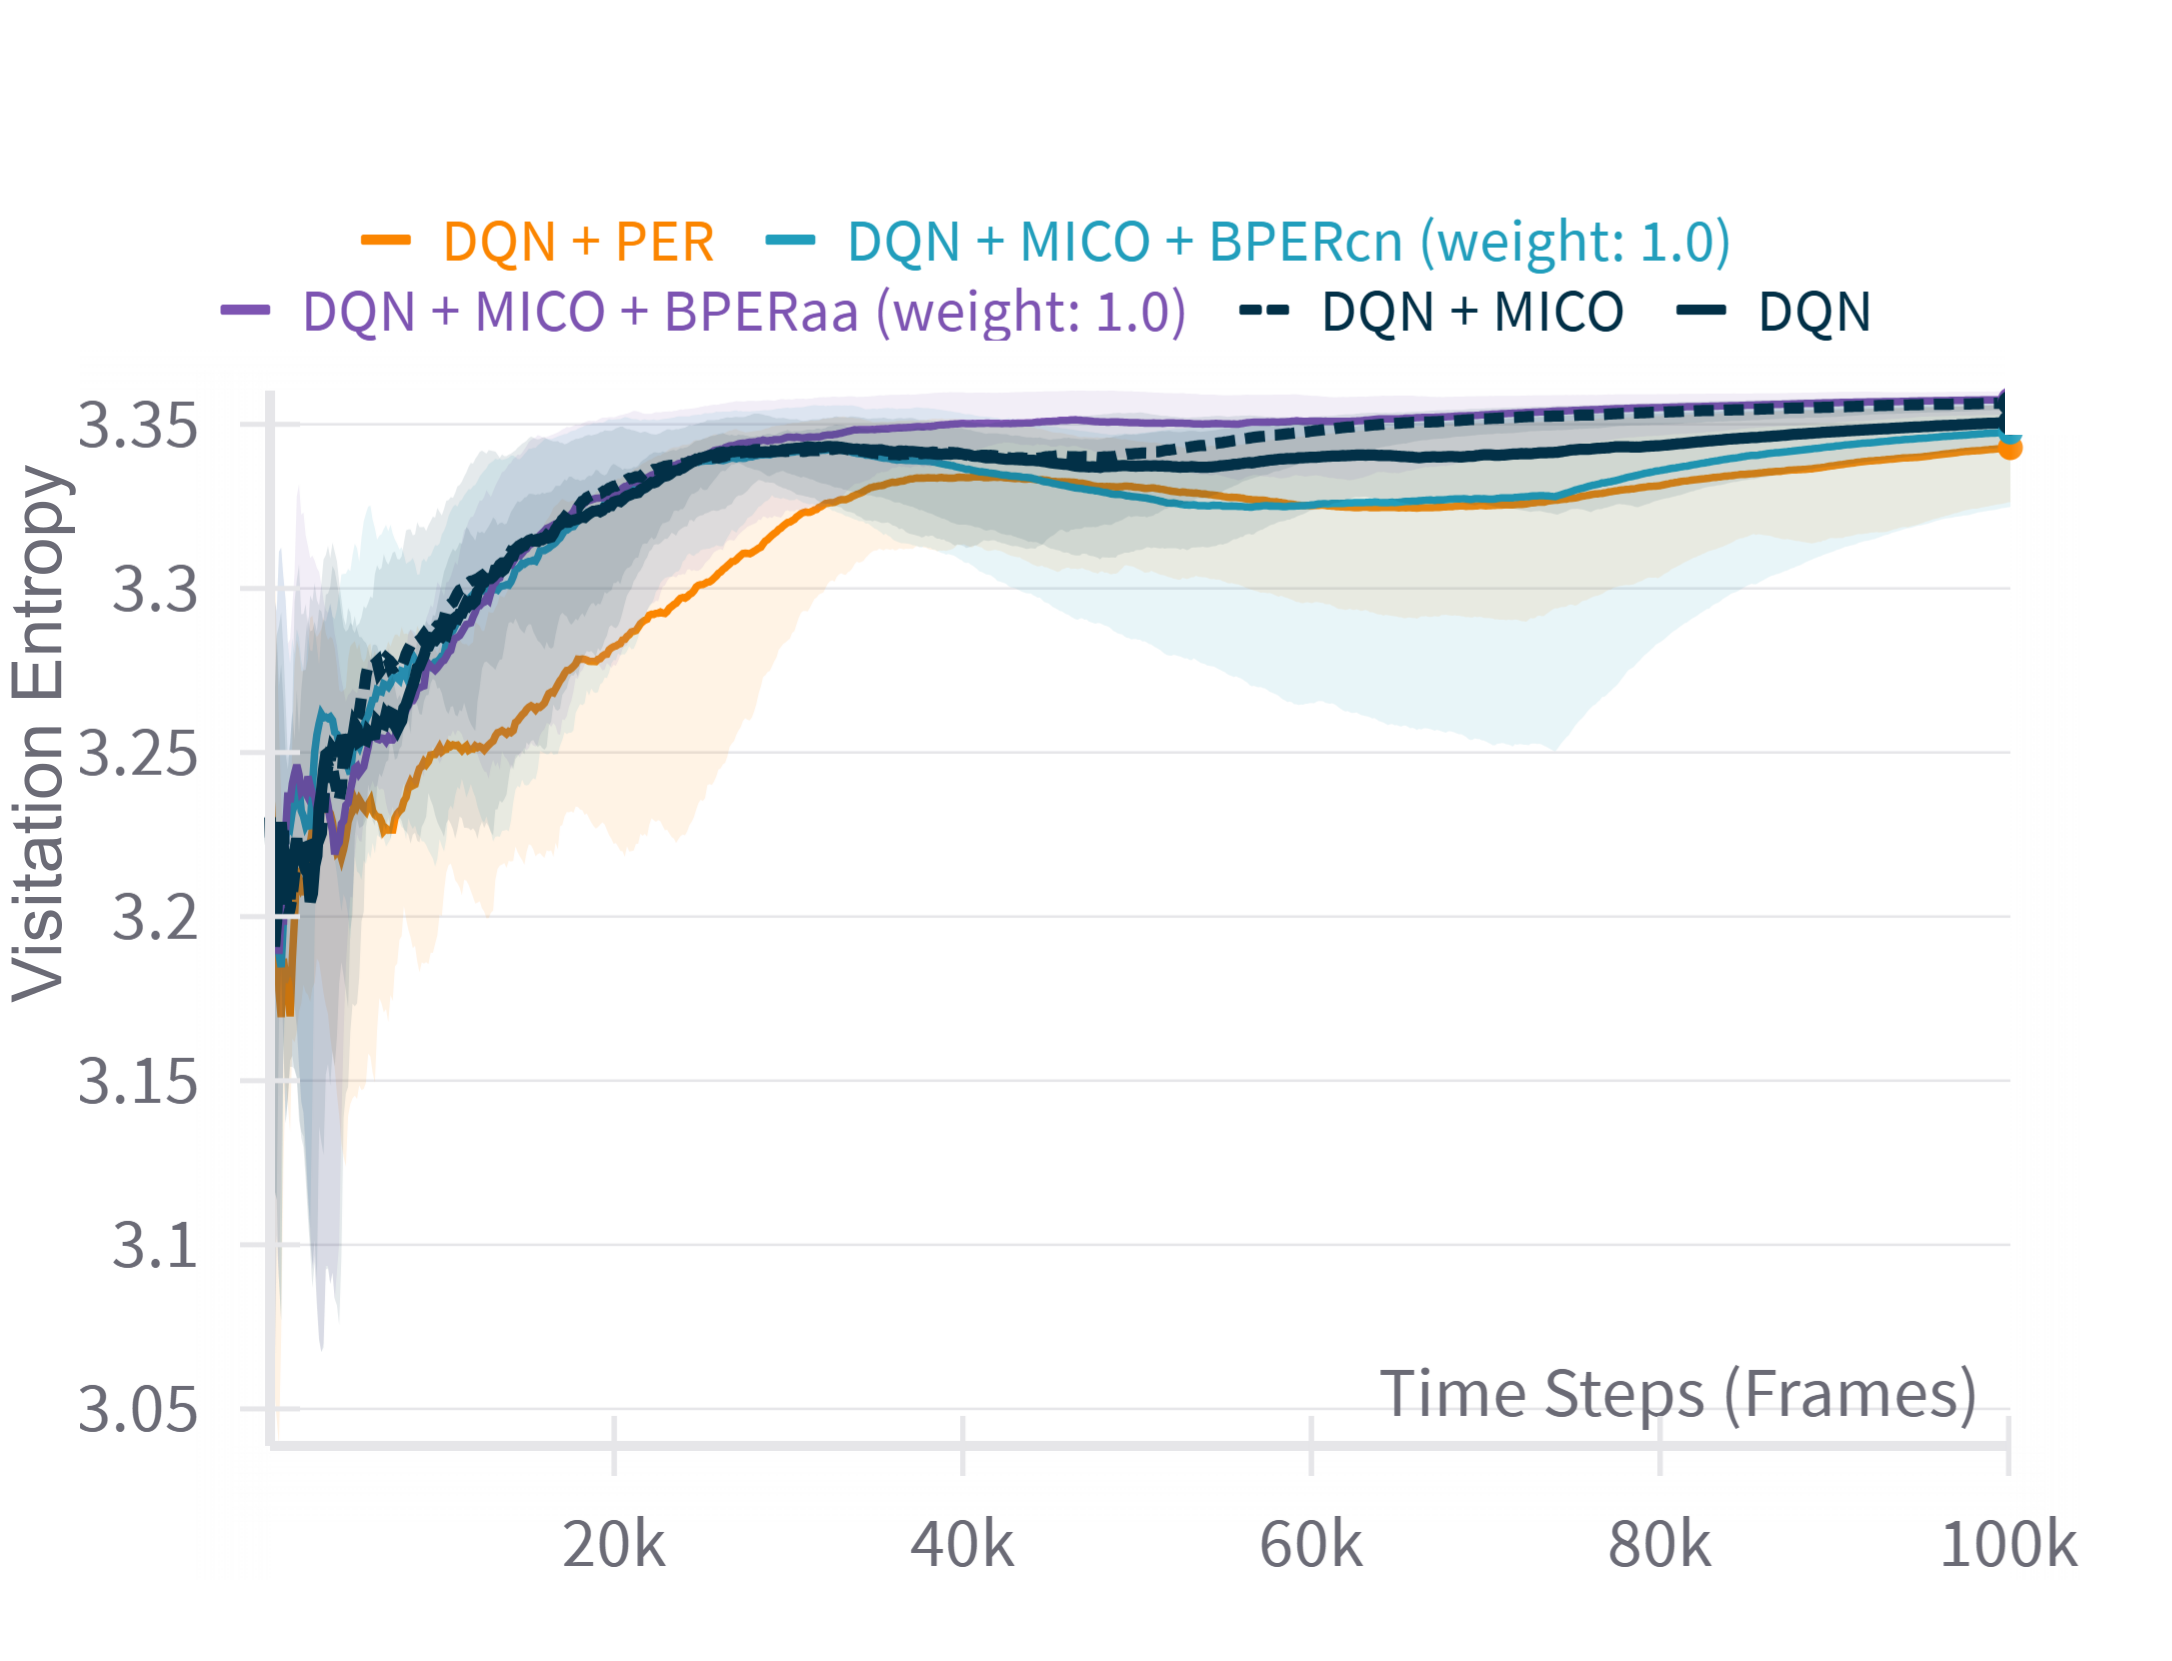
\includegraphics[width=1.\linewidth]{Results/grid_world/state_visitation_entropy.png}
    \caption{Caption}
    \label{fig:enter-label}
\end{figure}


\section{General RL Performance}


\begin{figure}[h]
    \centering
    \begin{subfigure}{0.45\textwidth}
    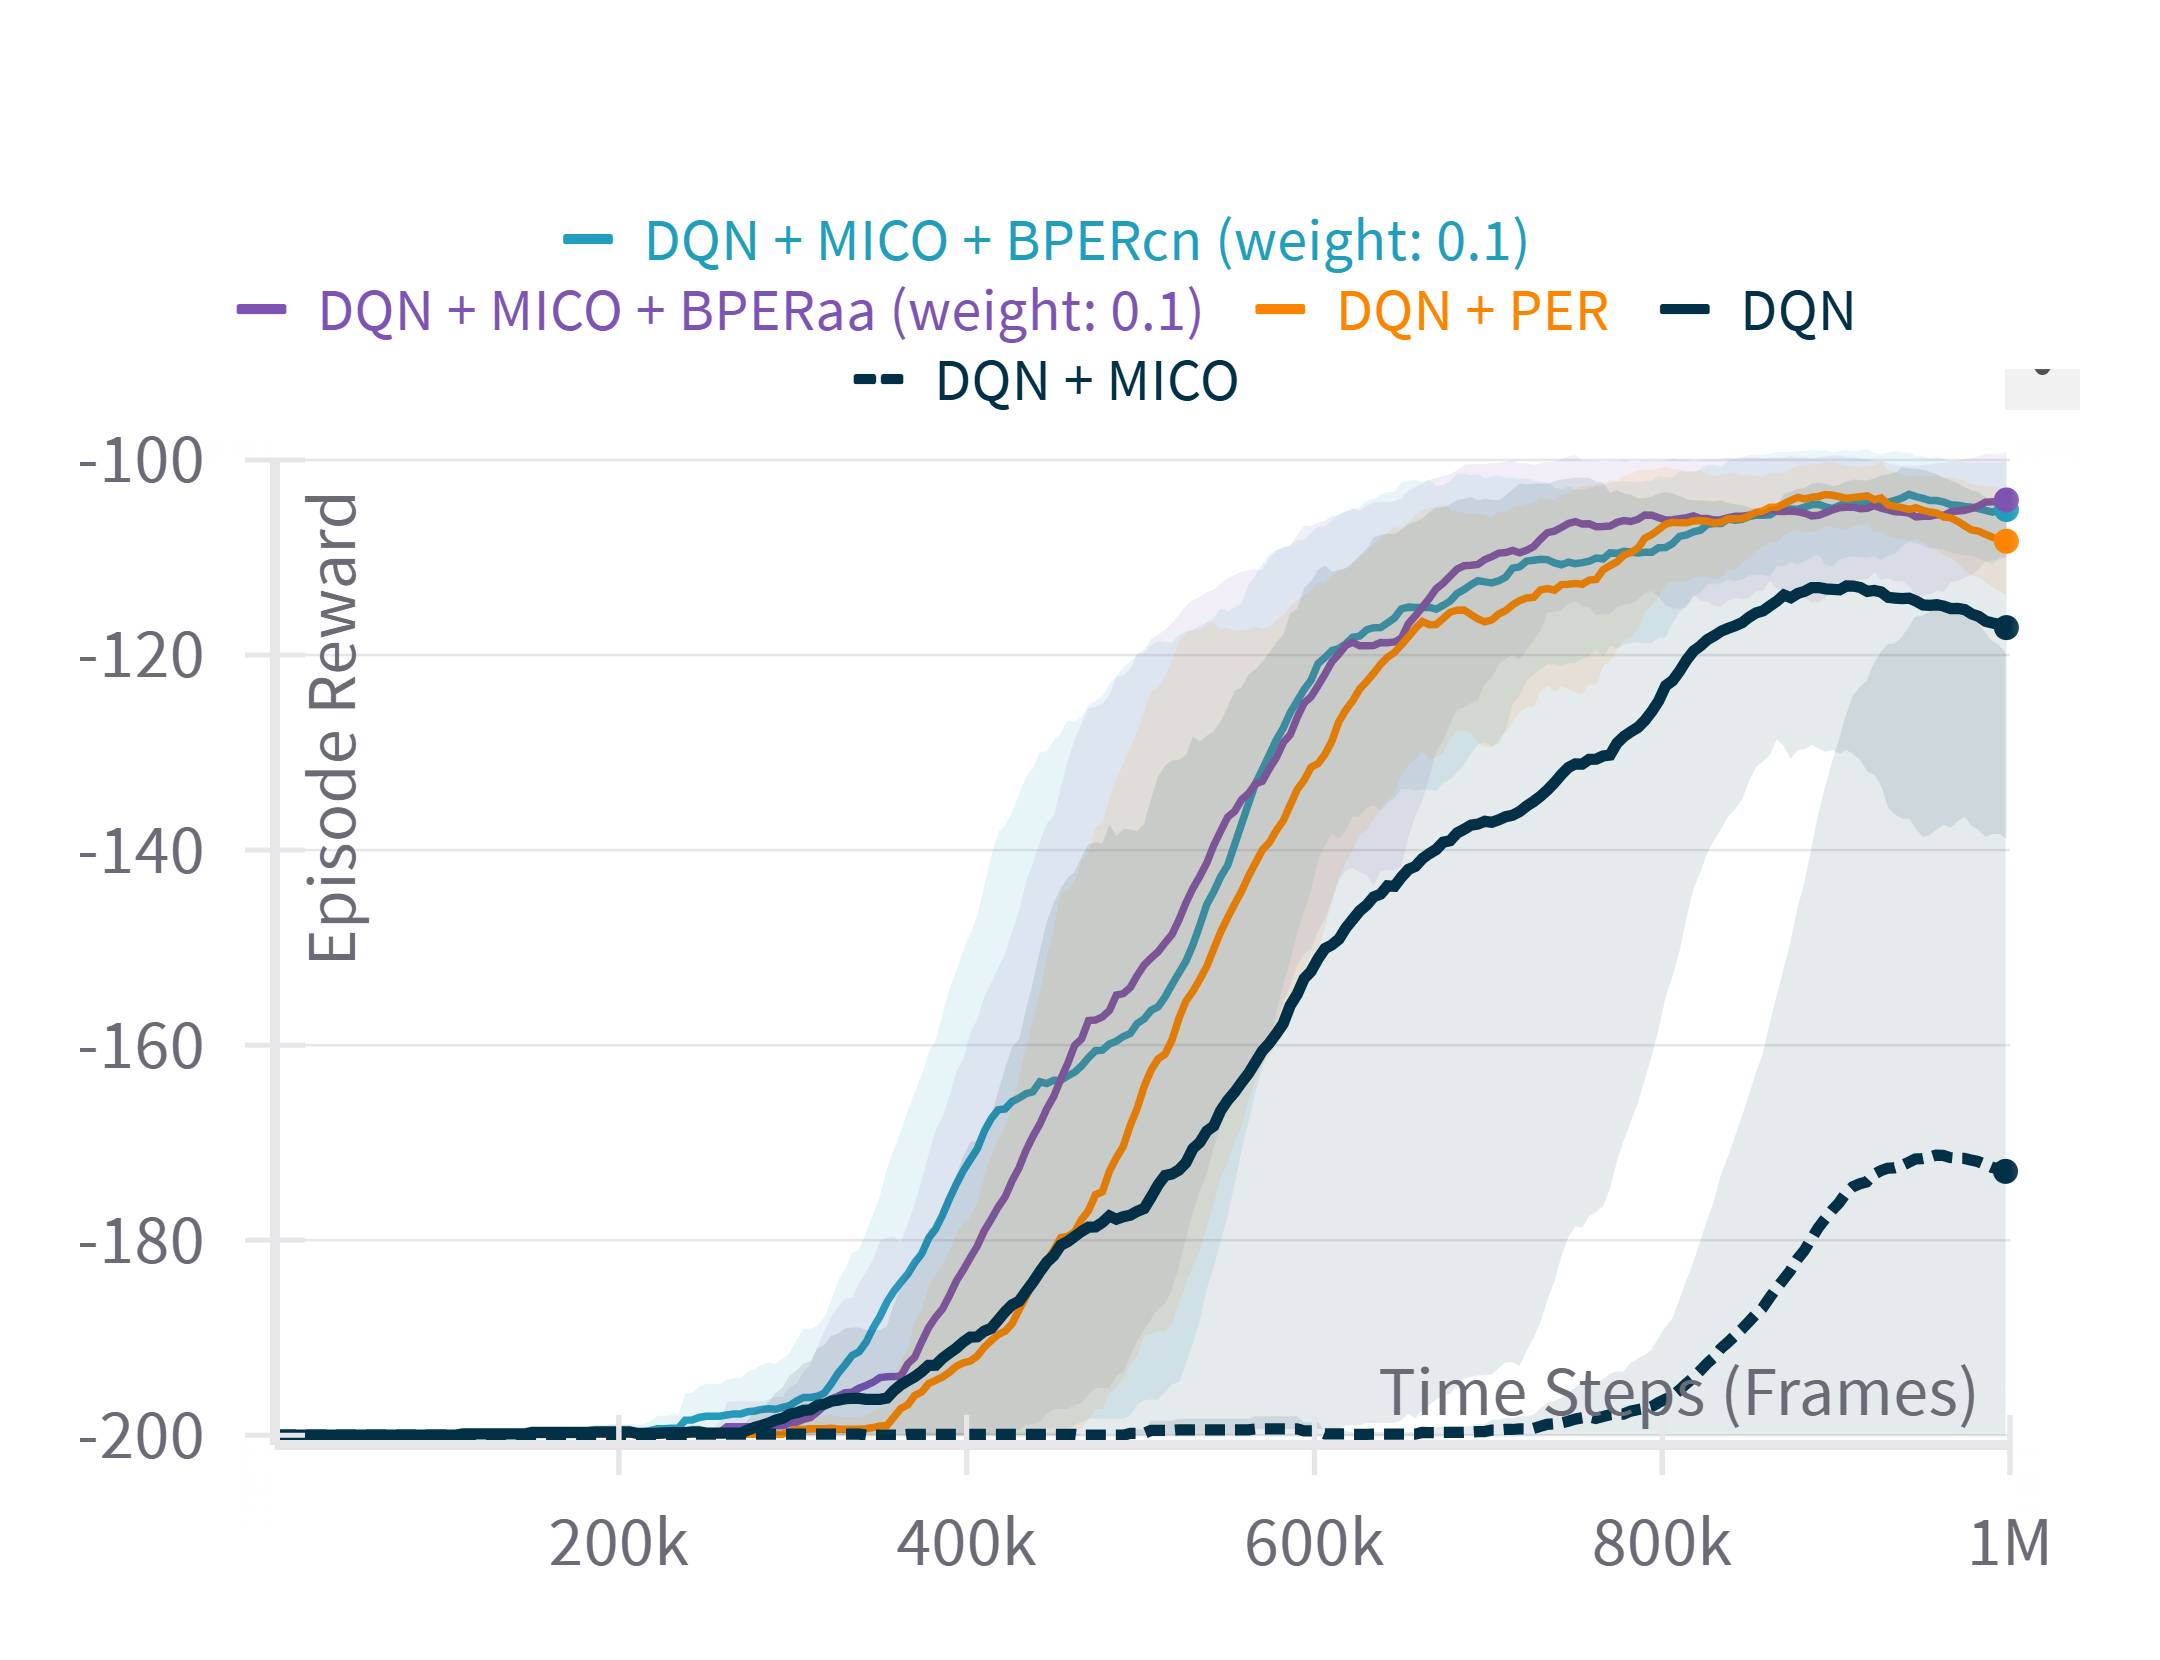
\includegraphics[width=\linewidth]{Results/general_results/episode_reward_mountaincarv0.png}
        \caption{MountainCar-v0}
        \label{fig:on_policy_weighting}
    \end{subfigure}
    \hfill
    \begin{subfigure}{0.45\textwidth}
        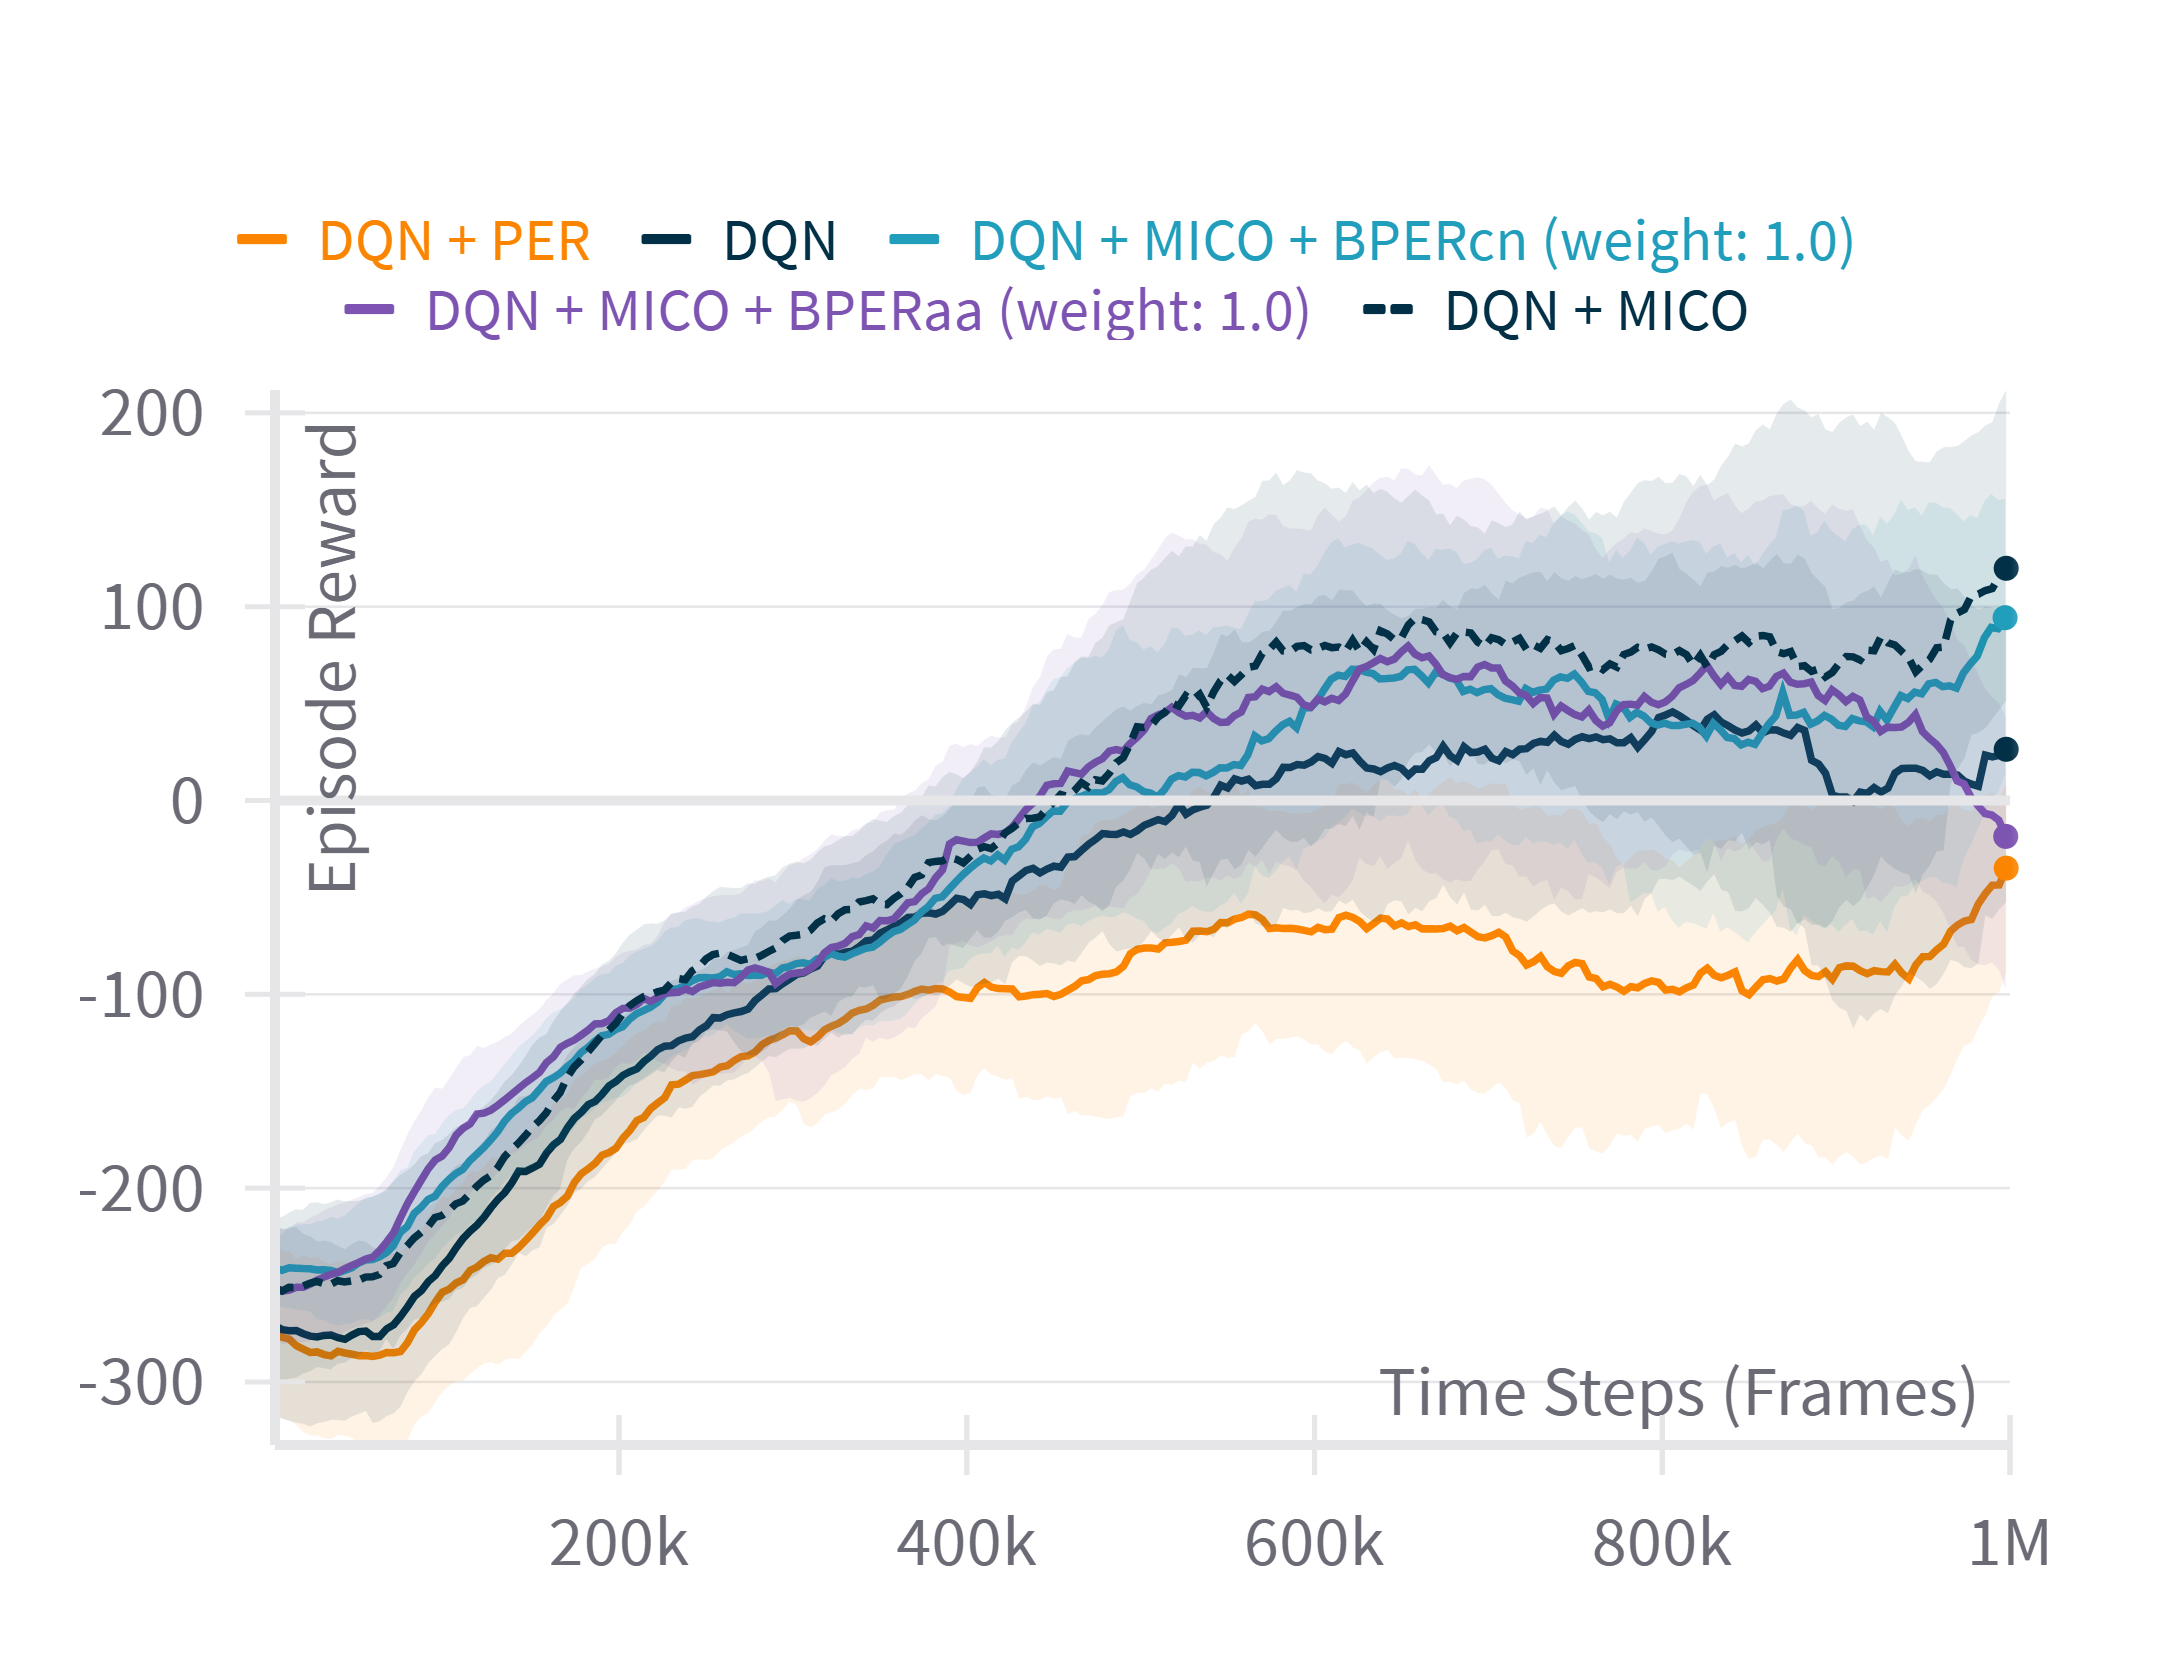
\includegraphics[width=\linewidth]{Results/general_results/episode_reward_lunarlander.png}
        \caption{LunarLander-v1}
        \label{fig:uniform_weighting}
    \end{subfigure}
    \hfill
    \begin{subfigure}{0.45\textwidth}
        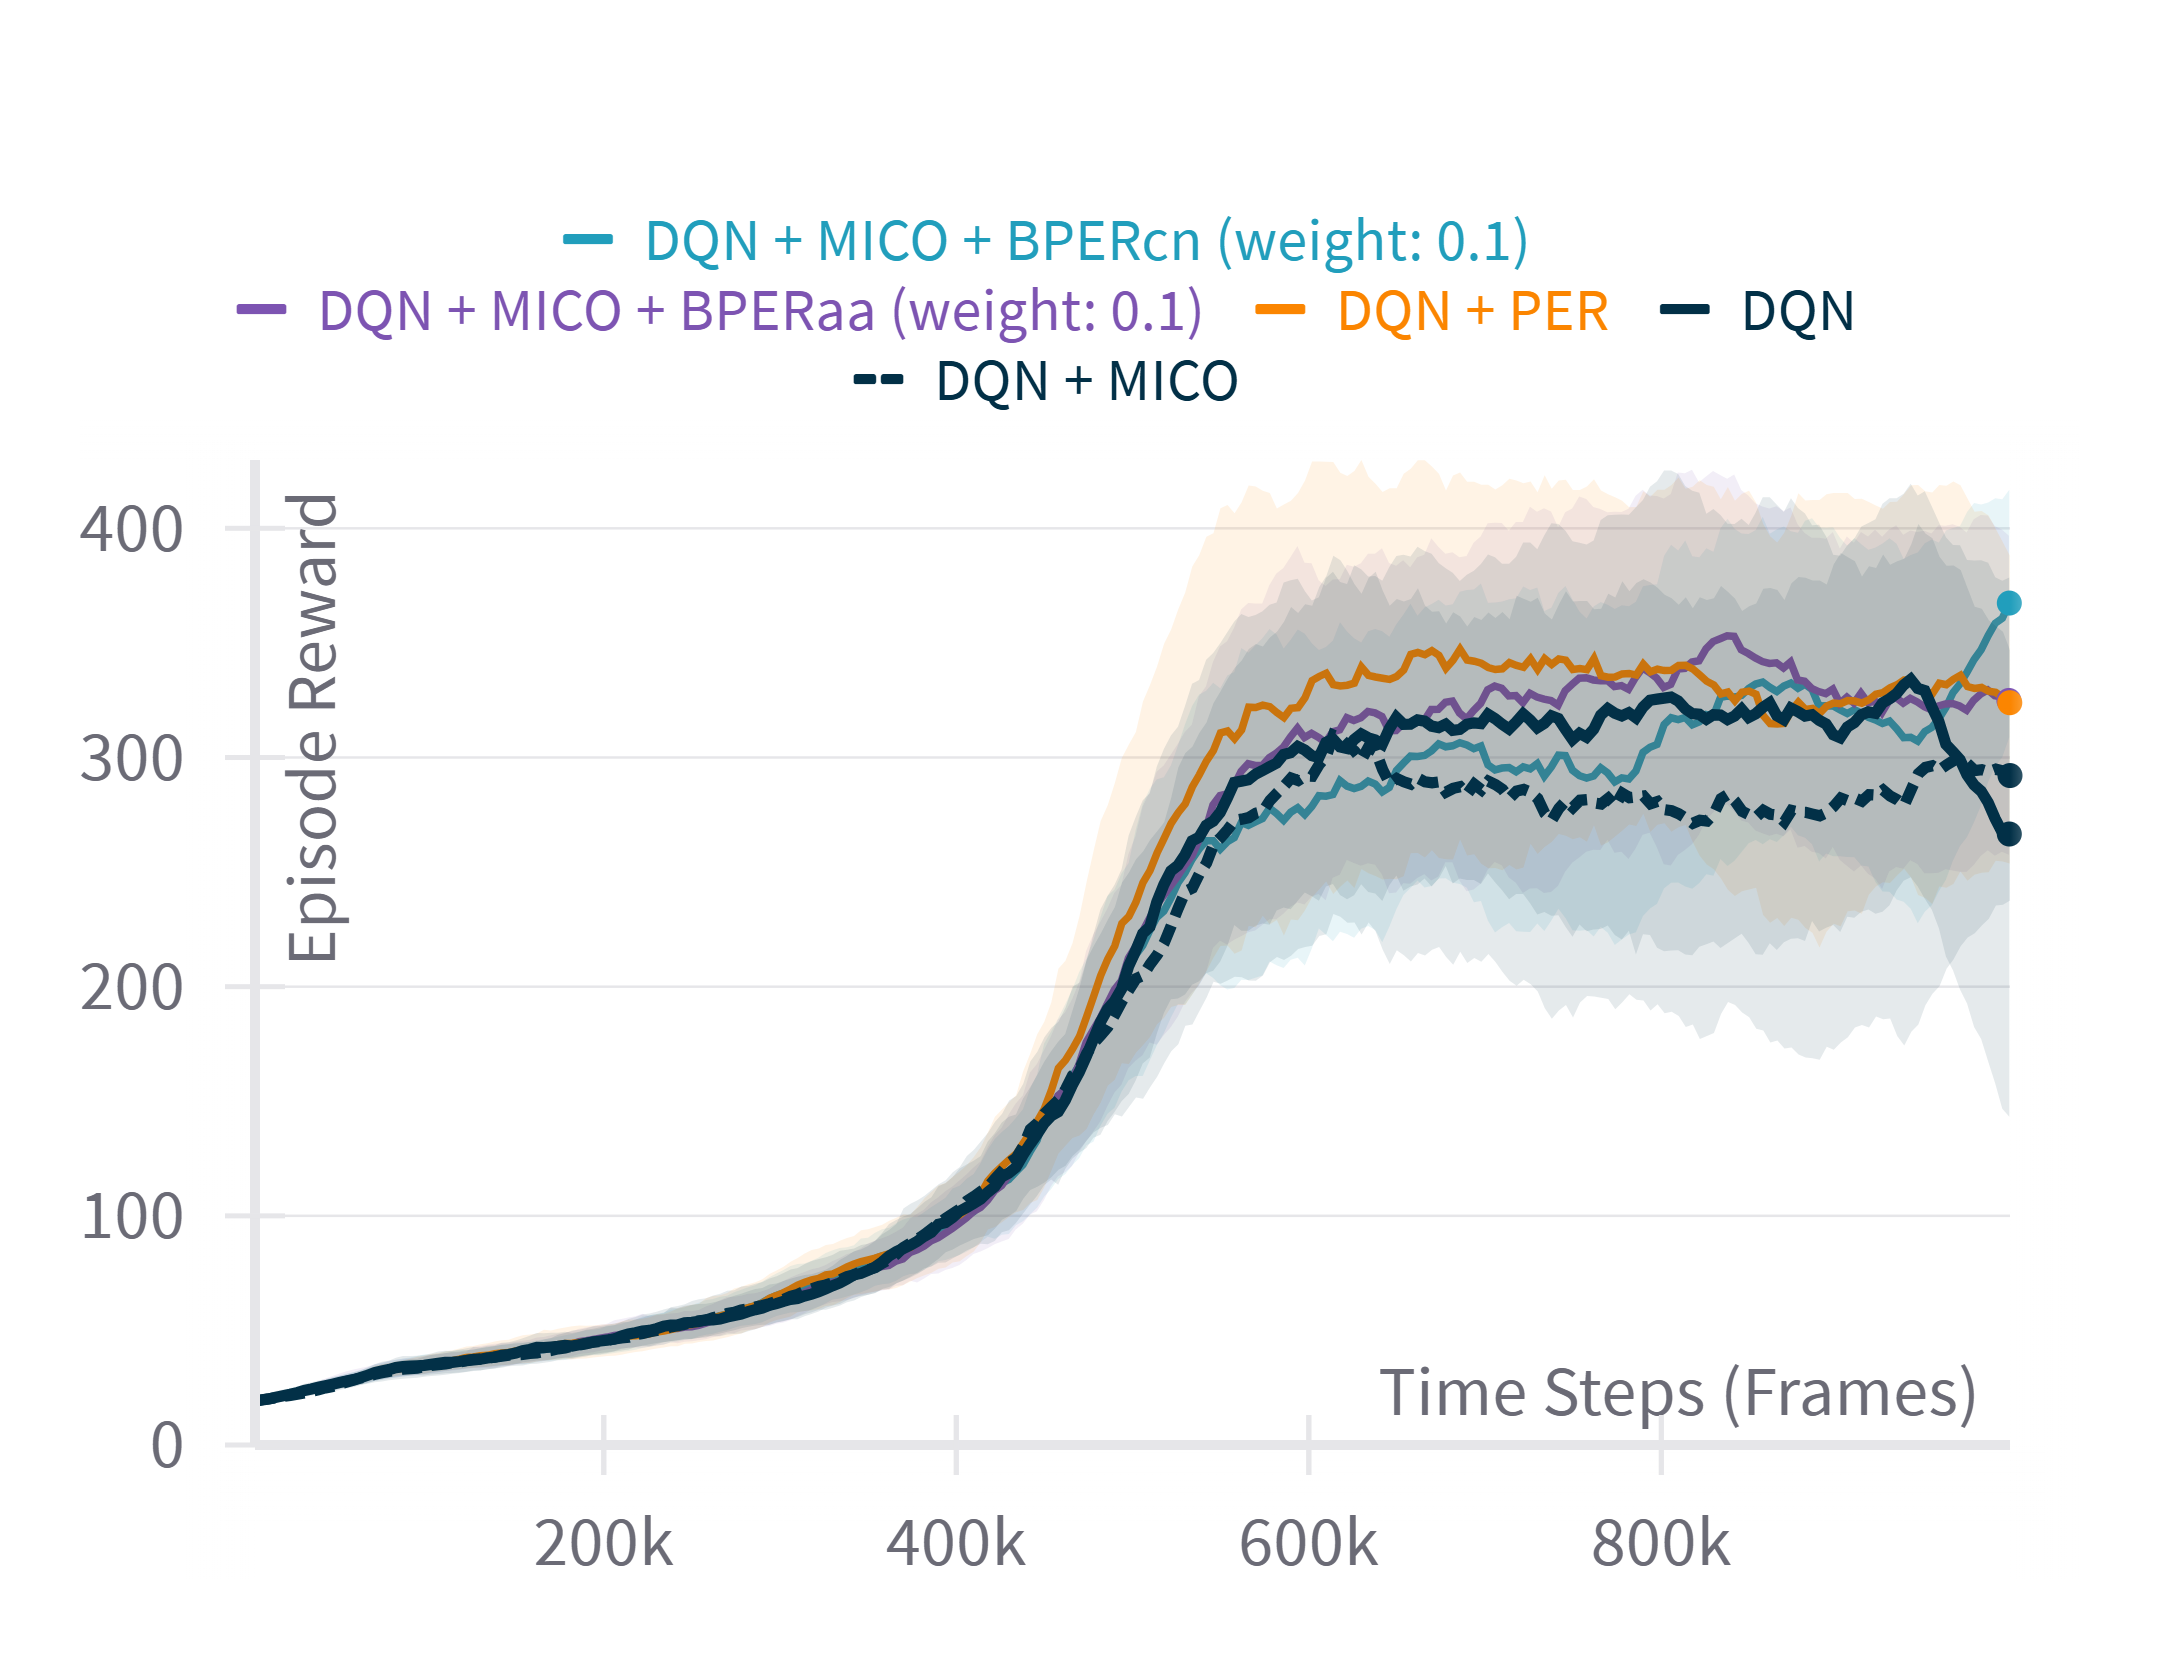
\includegraphics[width=\linewidth]{Results/general_results/episode_reward_cartpolev1.png}
        \caption{CartPole-v1}
        \label{fig:uniform_weighting}
    \end{subfigure}
    \hfill
    \begin{subfigure}{0.45\textwidth}
        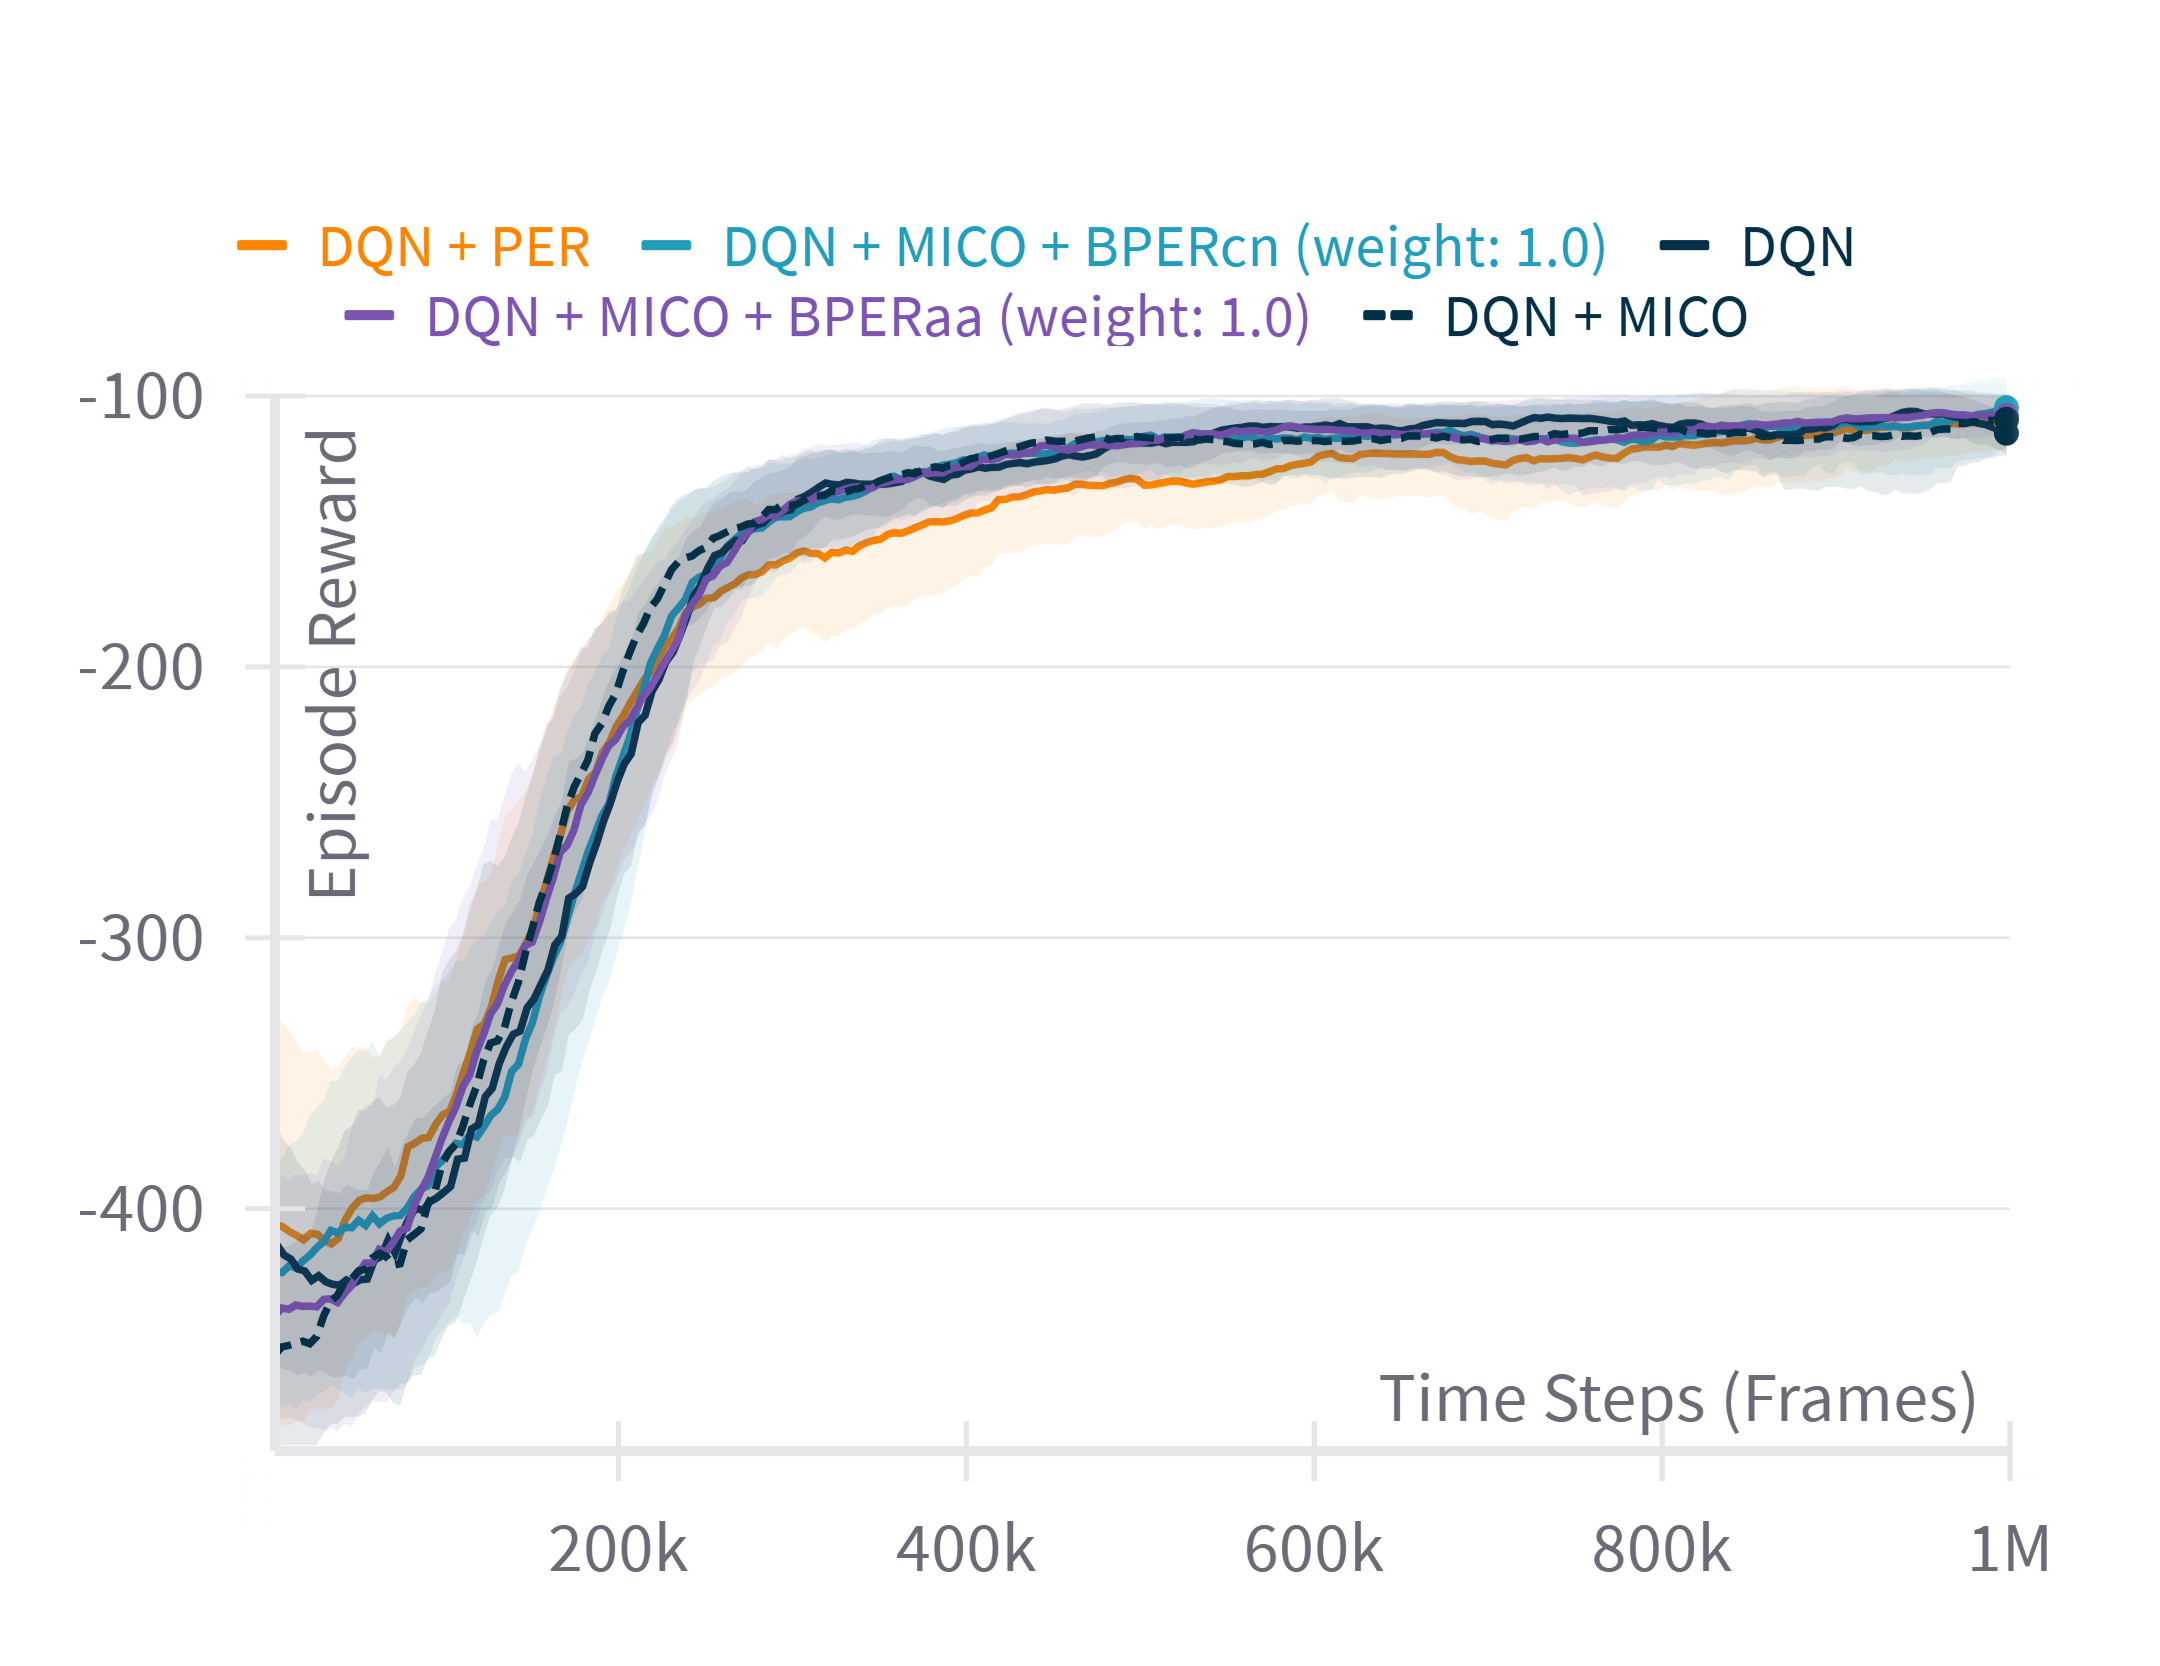
\includegraphics[width=\linewidth]{Results/general_results/episode_reward_acrobotv1.png}
        \caption{Acrobot-v1}
        \label{fig:uniform_weighting}
    \end{subfigure}
    \caption{Two images side-by-side}
    \label{fig:outdated_priorities}
\end{figure}

\begin{figure}[h]
    \centering
    \begin{subfigure}{0.45\textwidth}
    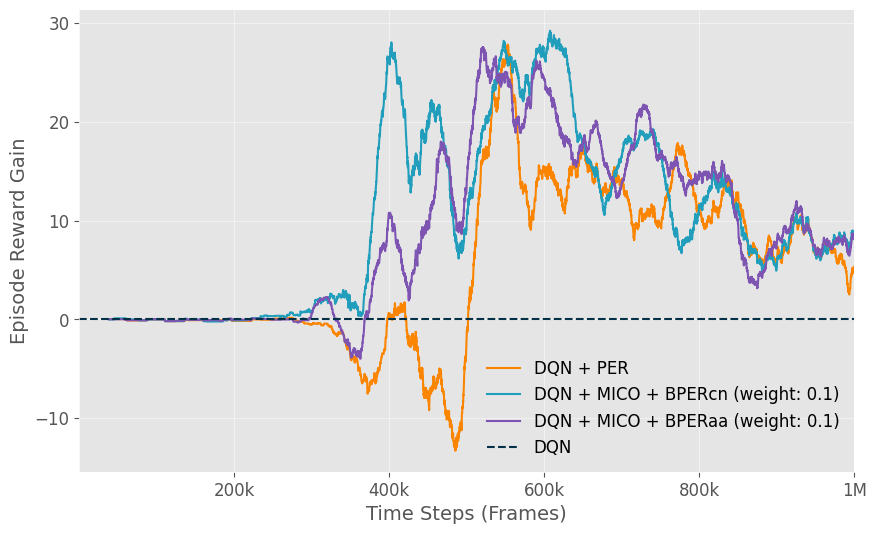
\includegraphics[width=\linewidth]{Results/general_results/mountain_car_reward_gain_vs_dqn.png}
        \caption{MountainCar-v0}
        \label{fig:on_policy_weighting}
    \end{subfigure}
    \hfill
    \begin{subfigure}{0.45\textwidth}
        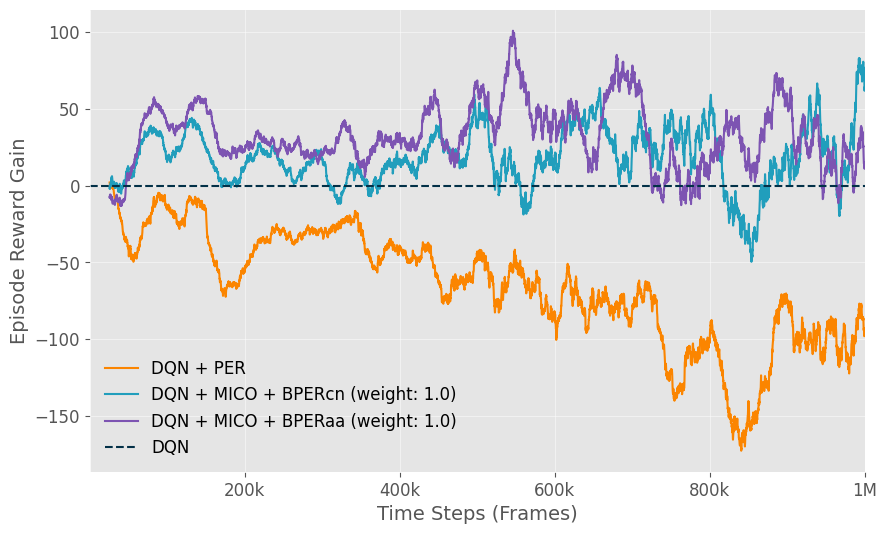
\includegraphics[width=\linewidth]{Results/general_results/lunarlander_reward_gain_vs_dqn.png}
        \caption{LunarLander-v1}
        \label{fig:uniform_weighting}
    \end{subfigure}
    \hfill
    \begin{subfigure}{0.45\textwidth}
        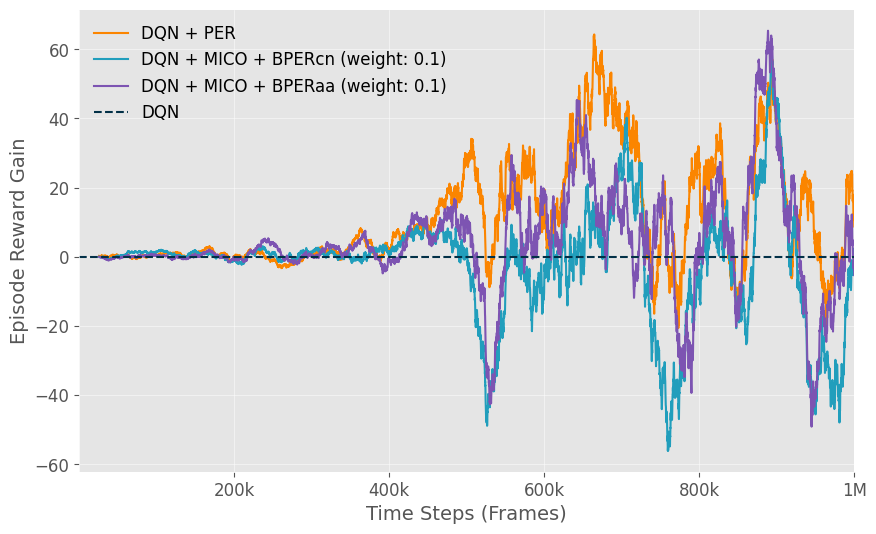
\includegraphics[width=\linewidth]{Results/general_results/cart_polev1_reward_gain_vs_dqn.png}
        \caption{CartPole-v1}
        \label{fig:uniform_weighting}
    \end{subfigure}
    \hfill
    \begin{subfigure}{0.45\textwidth}
        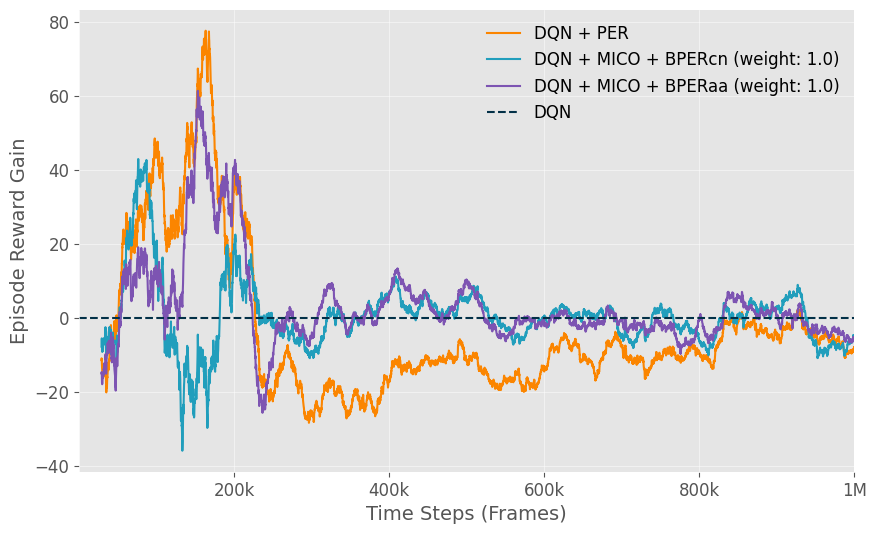
\includegraphics[width=\linewidth]{Results/general_results/acrobotv1_reward_gain_vs_dqn.png}
        \caption{Acrobot-v1}
        \label{fig:uniform_weighting}
    \end{subfigure}
    \caption{Two images side-by-side}
    \label{fig:outdated_priorities}
\end{figure}


% \begin{table}[h]
%     \centering
%     \caption{Performance Comparison of Different DQN Variants}
%     \label{tab:dqn_comparison}
%     \begin{tabular}{l >{\centering\arraybackslash}p{1.5cm} >{\centering\arraybackslash}p{1.5cm} >{\centering\arraybackslash}p{1.5cm} >{\centering\arraybackslash}p{1.5cm} >{\centering\arraybackslash}p{1.5cm} >{\centering\arraybackslash}p{1.5cm}}
%         \toprule
%                          & \multicolumn{2}{c}{\textbf{PER}}                       & \multicolumn{2}{c}{\textbf{BPERcn}}            & \multicolumn{2}{c}{\textbf{BPERaa}}             \\
%                          & {\color[HTML]{656565} \footnotesize DQN} & {\color[HTML]{656565} \footnotesize MICO} & {\color[HTML]{656565} \footnotesize DQN} & {\color[HTML]{656565} \footnotesize MICO} & {\color[HTML]{656565} \footnotesize DQN} & {\color[HTML]{656565} \footnotesize MICO} \\
%         \midrule
%         \textbf{MountainCar-v0} & $5.344 \pm 21.016$ & $39.088 \pm 39.151$   & $\mathbf{10.145} \pm \mathbf{21.471} $    & $\mathbf{43.889} \pm \mathbf{38.863}$  & $9.021 \pm 19.756$   & $42.765 \pm 39.060$     \\
%         \textbf{Cartpole-v1}    & $\mathbf{10.975} \pm \mathbf{133.140}$    & $\mathbf{24.23} \pm \mathbf{135.122}$   & $-2.100 \pm 134.322$   & $11.648 \pm 129.970$  & $3.790 \pm 134.959$    & $17.539 \pm 134.593$     \\
%         \textbf{Acrobot-v1}     & $-3.279 \pm 79.455$  & $-6.878 \pm 74.916$   & $0.250 \pm 78.057$    & $-3.350 \pm 73.122$  & $\mathbf{2.915} \pm \mathbf{75.618}$    & $\mathbf{-0.685} \pm \mathbf{70.853}$     \\
%         \textbf{LunarLander-v1} & $-65.620 \pm 175.613$    & $-107.075 \pm 183.781$   & $18.800 \pm 191.309$    & $-22.654 \pm 194.957$  & $\mathbf{32.125} \pm \mathbf{185.015}$    & $\mathbf{-9.330} \pm \mathbf{191.315}$   \\
%         \bottomrule
%     \end{tabular}
% \end{table}

\begin{table}[h]
    \hspace*{-1cm}
    \setlength{\tabcolsep}{2.5pt}
    \centering
    \begin{tabular}{llcccc}
        \toprule
        & \textbf{Baseline} & \textbf{MountainCar-v0} & \textbf{Cartpole-v1} & \textbf{Acrobot-v1} & \textbf{LunarLander-v1} \\
        \midrule
        {\footnotesize\textbf{PER}} & {\footnotesize\textbf{DQN}} & $5.344 \pm 21.016$ & $\mathbf{10.975} \pm \mathbf{133.140}$ & $-3.279 \pm 79.455$ & $-65.620 \pm 175.613$ \\
         & {\footnotesize\textbf{MICO}} & $39.088 \pm 39.151$ & $\mathbf{24.23} \pm \mathbf{135.122}$ & $-6.878 \pm 74.916$ & $-107.075 \pm 183.781$ \\
        {\footnotesize\textbf{BPERcn}} & {\footnotesize\textbf{DQN}} & $\mathbf{10.145} \pm \mathbf{21.471}$ & $-2.100 \pm 134.322$ & $0.250 \pm 78.057$ & $18.800 \pm 191.309$ \\
        & {\footnotesize\textbf{MICO}} & $\mathbf{43.889} \pm \mathbf{38.863}$ & $11.648 \pm 129.970$ & $-3.350 \pm 73.122$ & $-22.654 \pm 194.957$ \\
        {\footnotesize\textbf{BPERaa}} & {\footnotesize\textbf{DQN}} & $9.021 \pm 19.756$ & $3.790 \pm 134.959$ & $\mathbf{2.915} \pm \mathbf{75.618}$ & $\mathbf{32.125} \pm \mathbf{185.015}$ \\
        & {\footnotesize\textbf{MICO}} & $42.765 \pm 39.060$ & $17.539 \pm 134.593$ & $\mathbf{-0.685} \pm \mathbf{70.853}$ & $\mathbf{-9.330} \pm \mathbf{191.315}$ \\
        \bottomrule
    \end{tabular}
    \caption{Performance Comparison of Different DQN Variants}
    \label{tab:dqn_comparison_transposed}
\end{table}

\begin{figure}[h]
    \centering
    \begin{subfigure}{0.45\textwidth}
    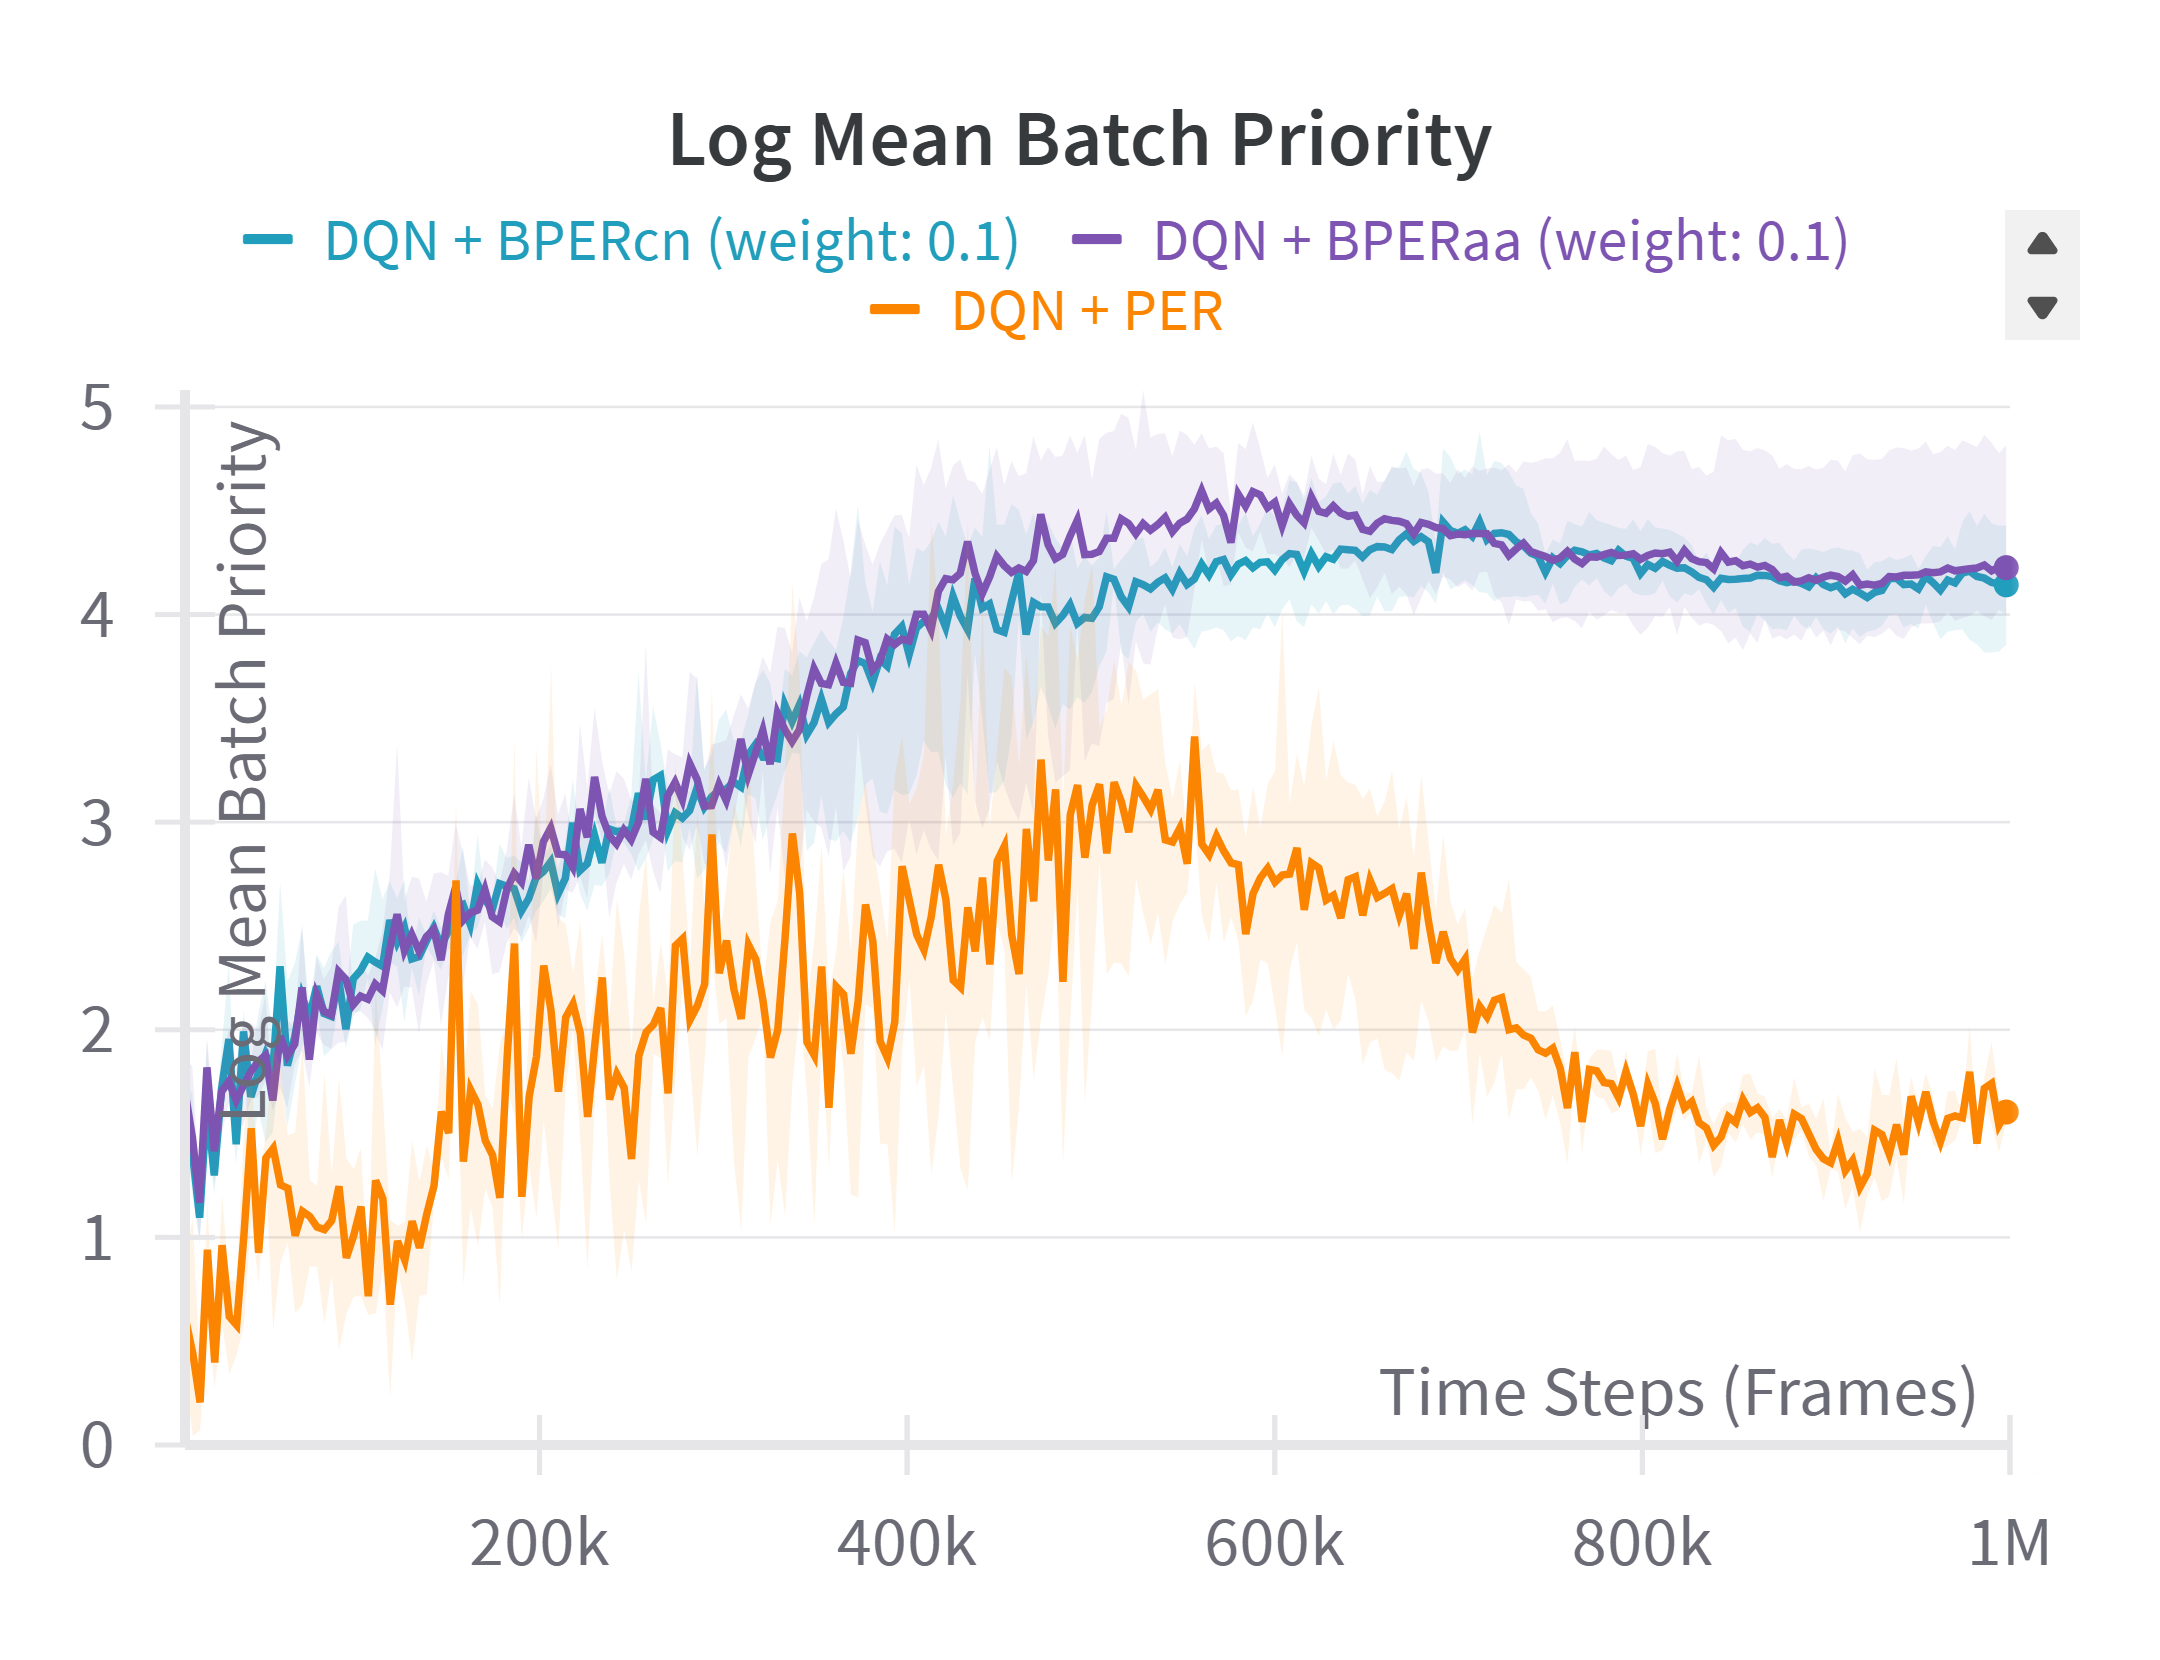
\includegraphics[width=\linewidth]{Results/general_results/log_mean_batch_priority_mountain_car.png}
        \caption{MountainCar-v0}
        \label{fig:on_policy_weighting}
    \end{subfigure}
    \hfill
    \begin{subfigure}{0.45\textwidth}
        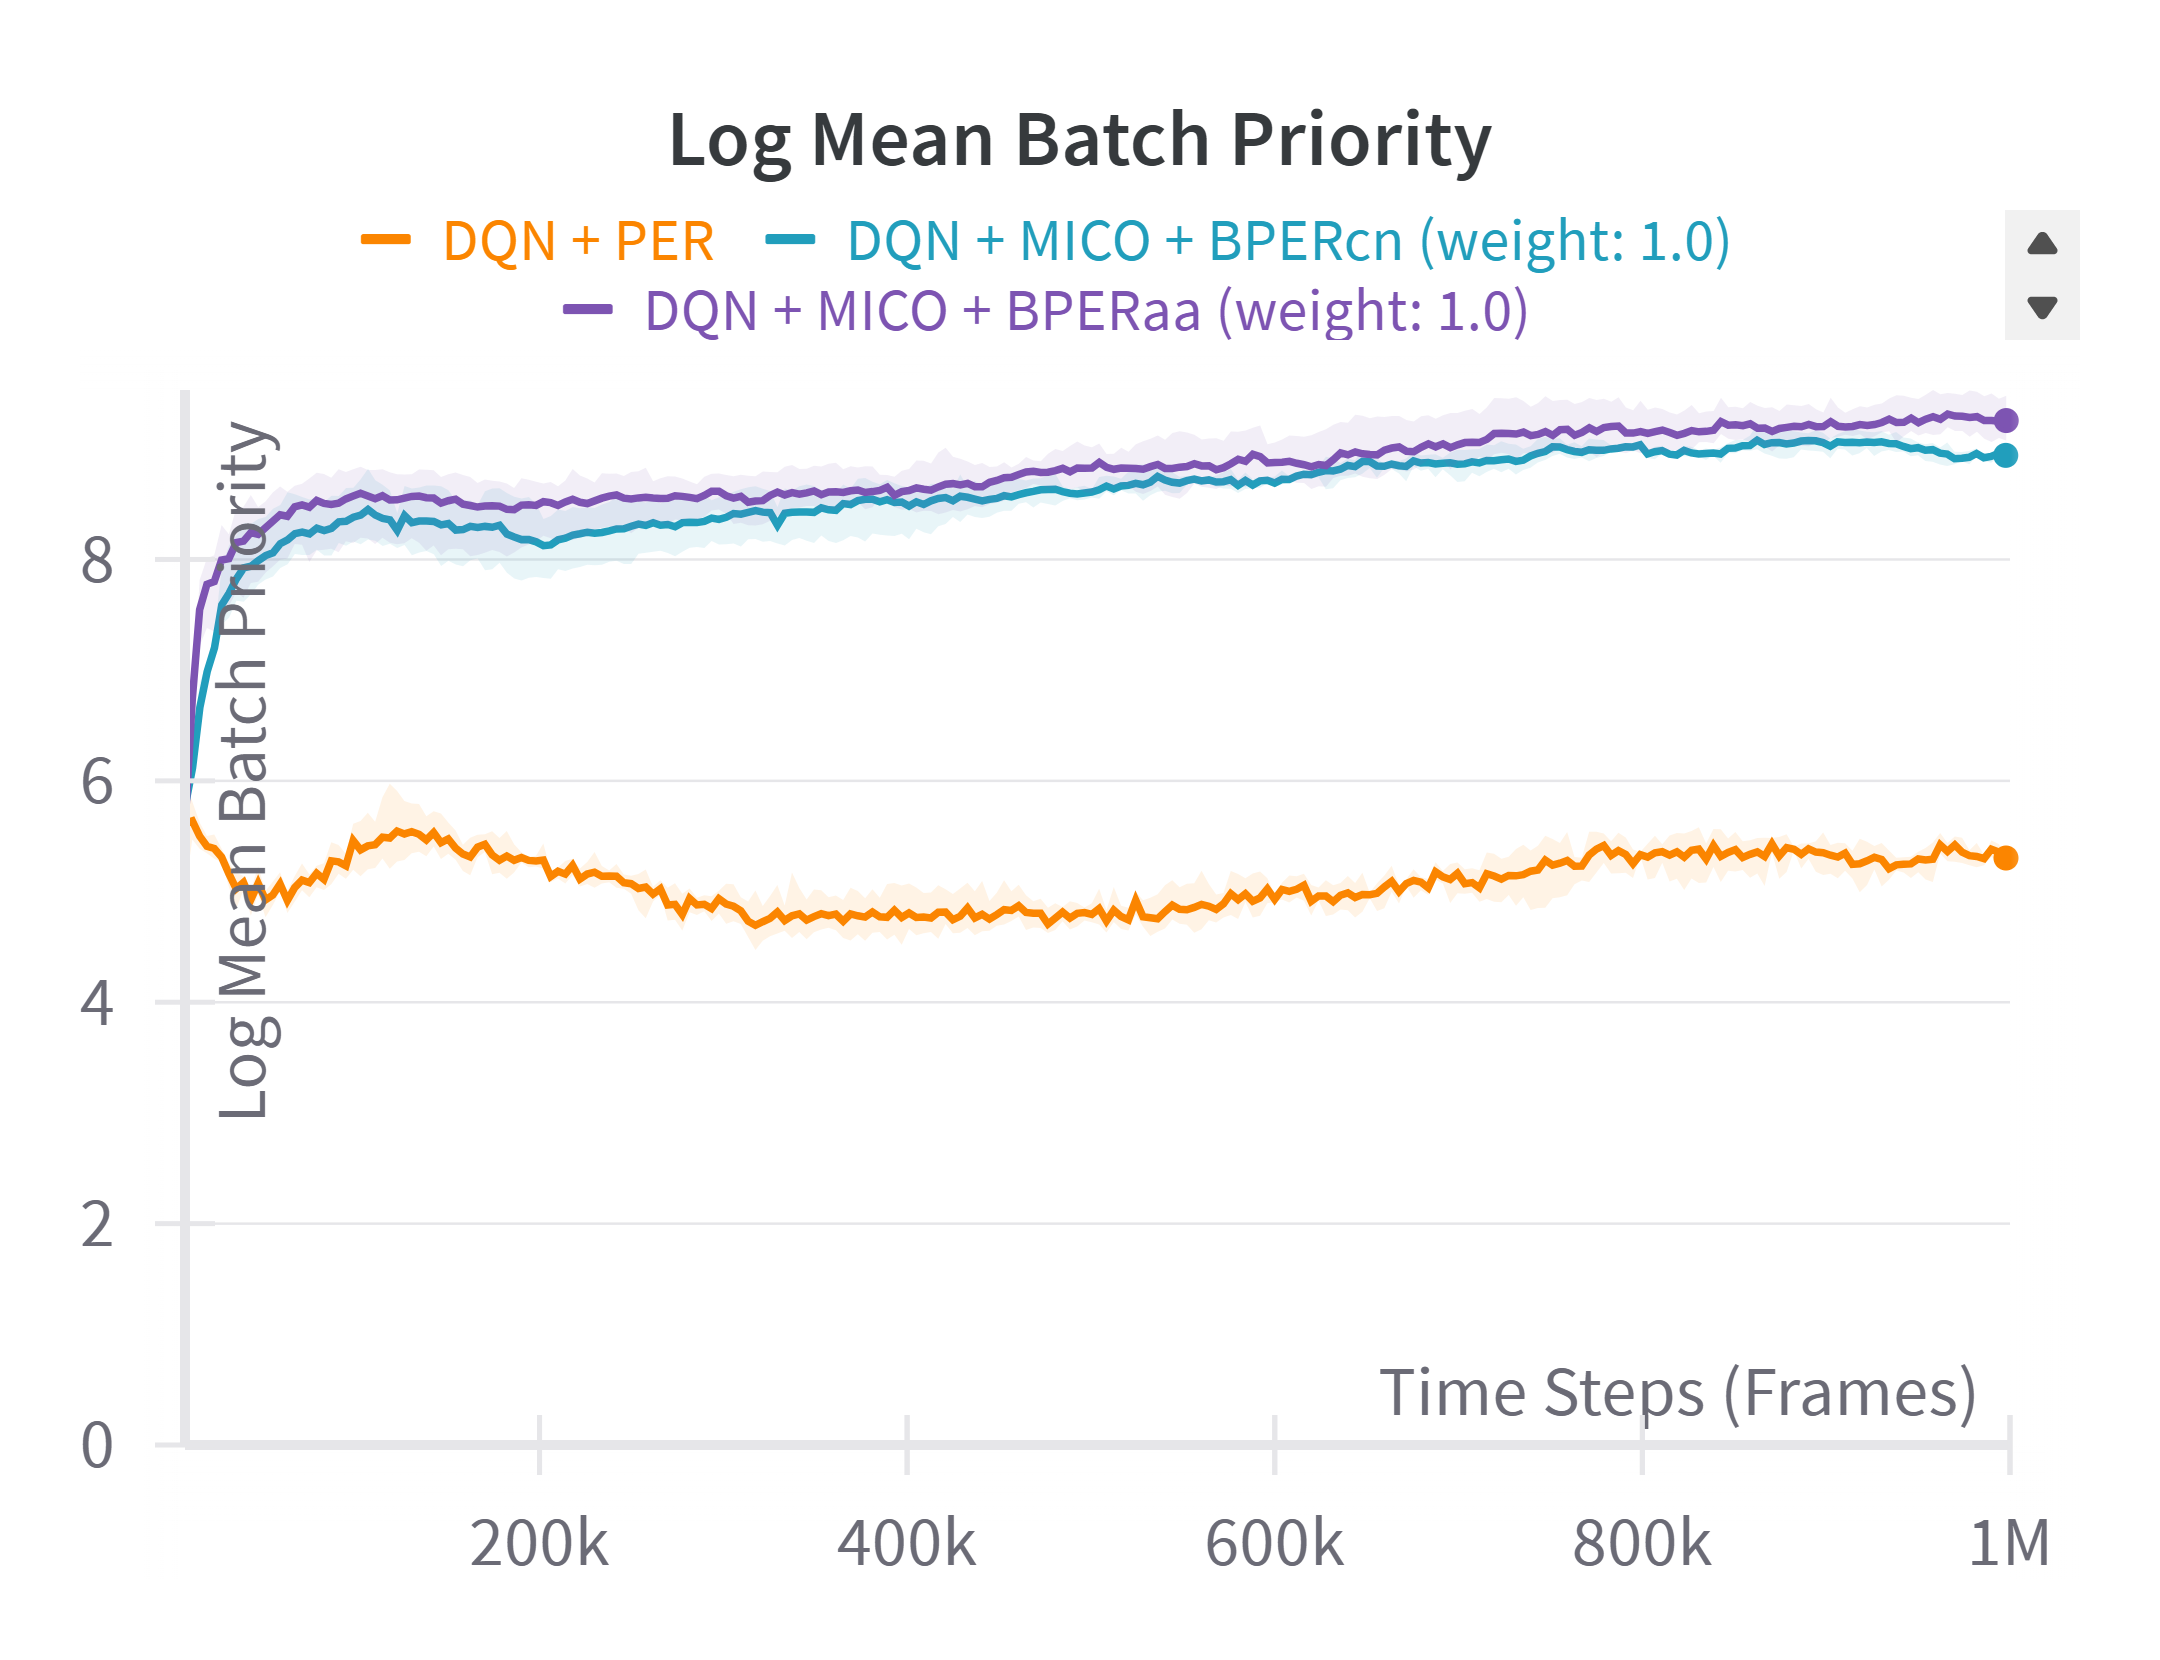
\includegraphics[width=\linewidth]{Results/general_results/log_mean_batch_priority_lunarlander.png}
        \caption{LunarLander-v1}
        \label{fig:uniform_weighting}
    \end{subfigure}
    \hfill
    \begin{subfigure}{0.45\textwidth}
        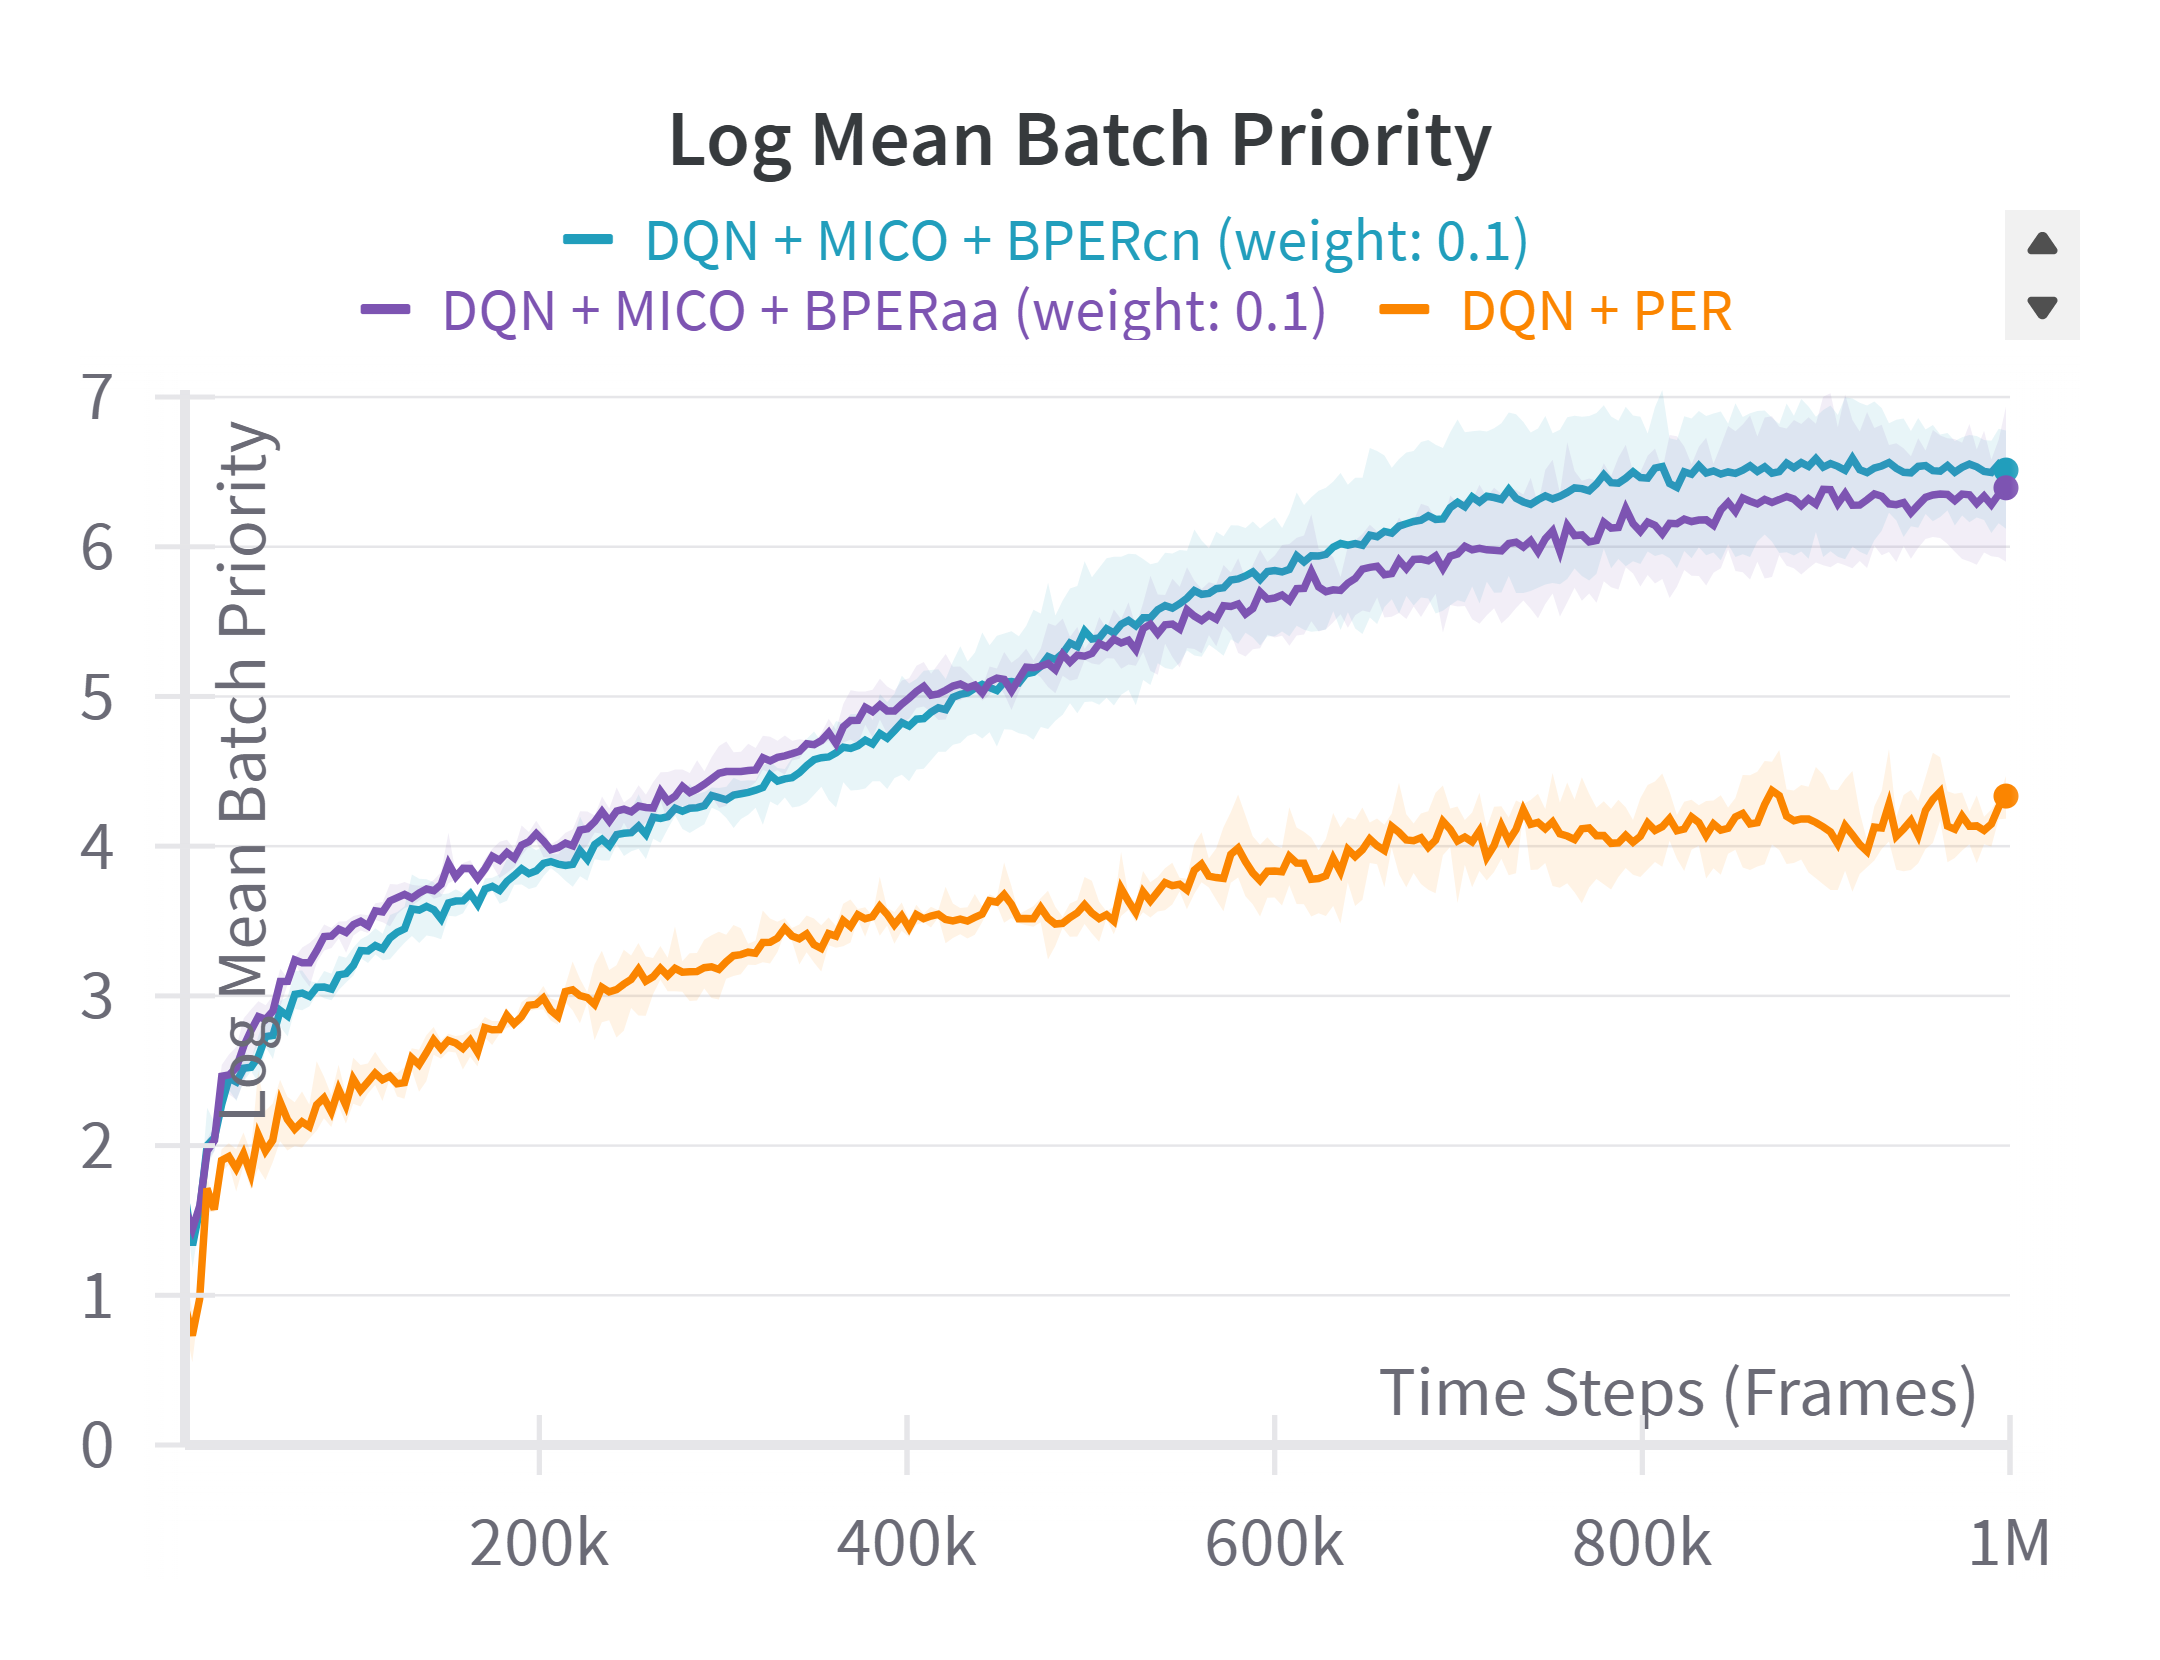
\includegraphics[width=\linewidth]{Results/general_results/log_mean_batch_priority_cartpolev1.png}
        \caption{CartPole-v1}
        \label{fig:uniform_weighting}
    \end{subfigure}
    \hfill
    \begin{subfigure}{0.45\textwidth}
        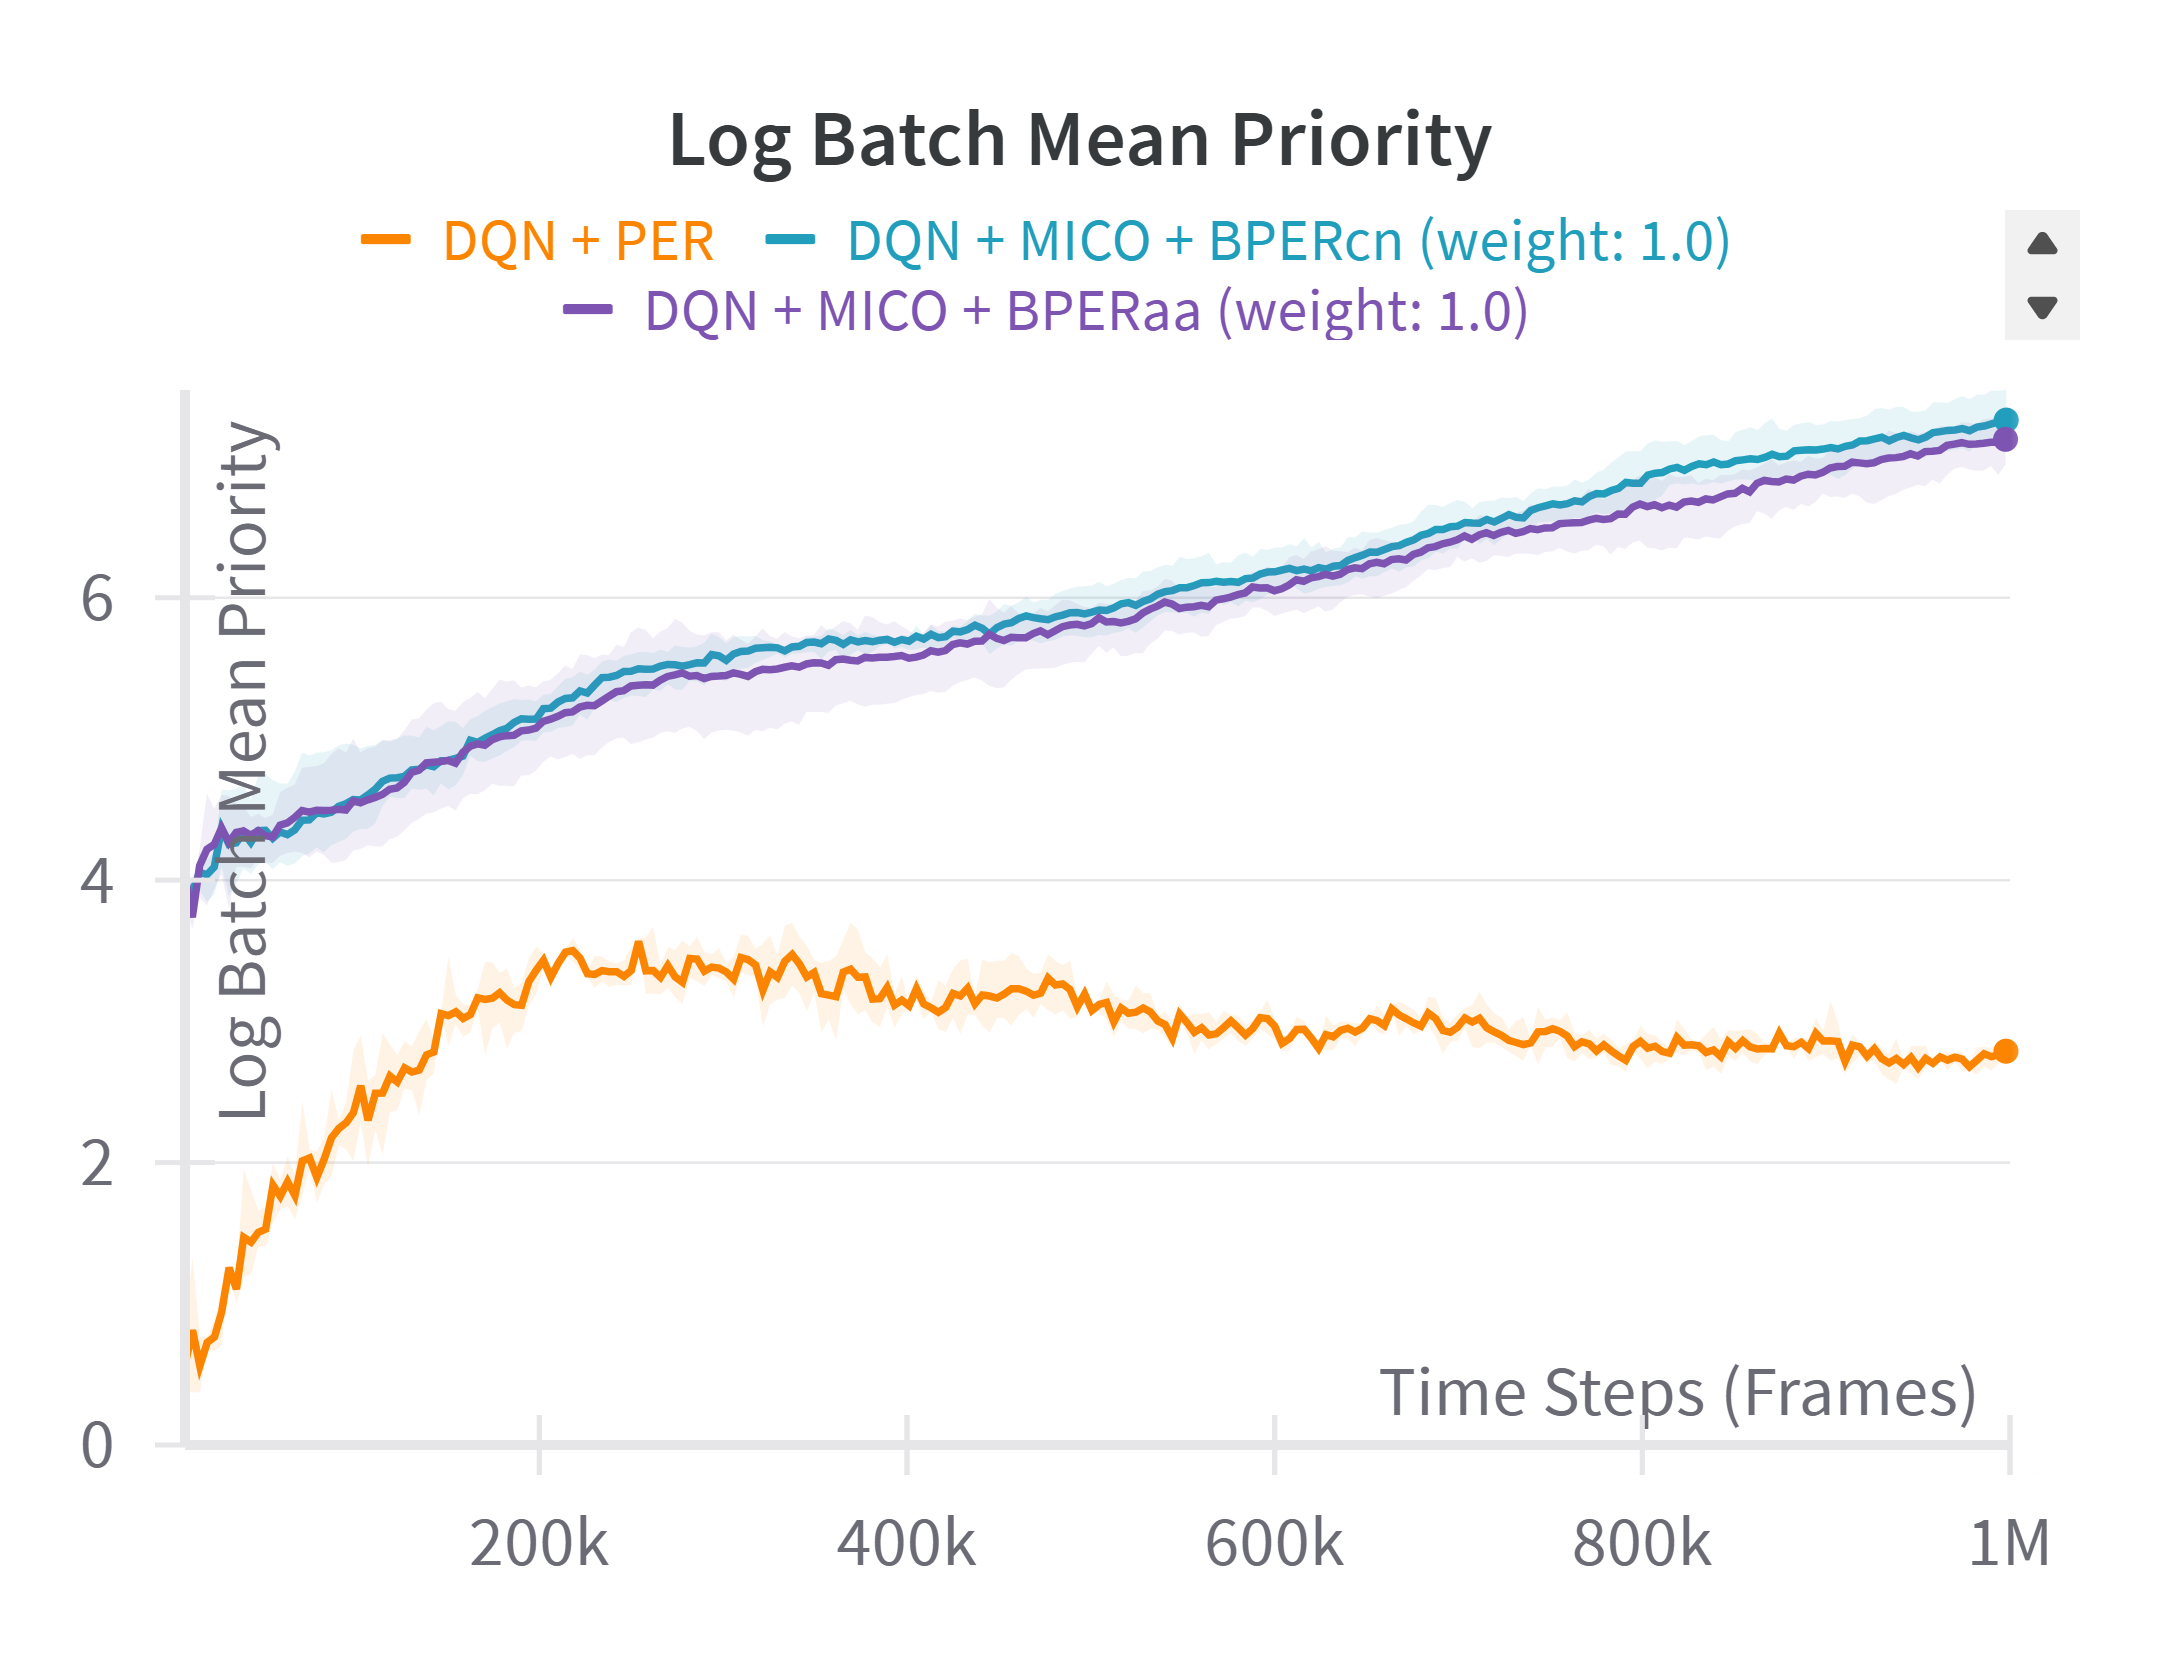
\includegraphics[width=\linewidth]{Results/general_results/log_mean_batch_priority_acrobot.png}
        \caption{Acrobot-v1}
        \label{fig:uniform_weighting}
    \end{subfigure}
    \caption{Two images side-by-side}
    \label{fig:outdated_priorities}
\end{figure}
